\documentclass[../main.tex]{subfiles}
\begin{document}
\section{定位问题}
\subsection{定位问题的基本概念}
\begin{enumerate}
    \item \textbf{定位}:确定机器人在\textbf{世界}(全局)坐标系中的位置/位姿
\end{enumerate}
\subsection{基于外部设备感知的定位}
\begin{enumerate}
    \item \textbf{全球定位系统GPS}
    \begin{itemize}
        \item \textbf{GPS(Global Positioning System)}:由\textbf{空间端}\footnote{24颗卫星位于6个倾角为55度的轨道平面内,每个轨道平面内4颗卫星,高度20182千米,周期12小时}、\textbf{控制端}\footnote{包括1个主控站、1个备用主控站、4个地面天线站和6个监测站,主要作用监测控制卫星的运行,并对卫星进行时间同步}和\textbf{用户端}\footnote{卫星接收到信号,根据信号发射时间和接收时间差计算接收器和卫星之间的距离}三部分组成,也称为GNSS (Global Navigation Satellite System)
            \begin{figure}[H]
                \centering
                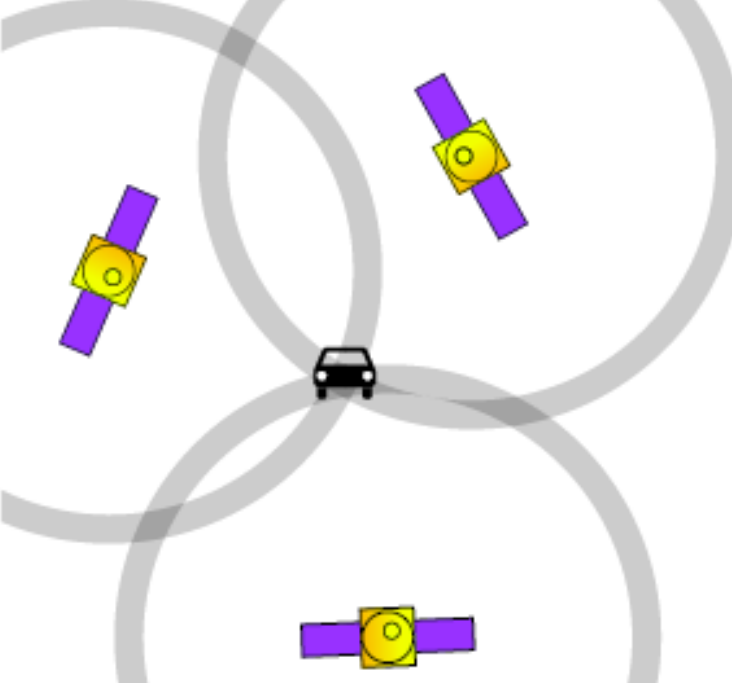
\includegraphics[width=0.3\textwidth]{images/gps.png}
                \caption{三点定位法}
            \end{figure}
        {\small\kaishu Q:为什么至少需要四个卫星的信号实现最优估计?\\A:电磁波传播速度等同于光束,因此,
时钟精度会极大地影响定位精度:
    \begin{itemize}
        \item 卫星时钟采用原子钟,精度高
        \item 接收器时钟采用石英钟,通常不够精确
    \end{itemize}
在估计用户端位置时,有必要同时估计接收器时钟误差,即估计状态为\( \mathbf{x} = {\left( x,y,z,{\delta }_{\text{clock }}\right) }^{T} \)}
        \item \textbf{差分全球定位系统 DGPS (DIFFERENTIAL GPS)}:消除GPS系统中出于利益考虑被人为引入的误差,基本原理是:
            \begin{itemize}
                \item 在位置精确测定的已知点上配备一台GPS接收机作为基准站
                \item 基准站将GPS观测结果与基准站坐标比较,求解出\textbf{实时差分修正值},广播给附近用户
            \end{itemize}
        \item \textbf{缺点}:
        \begin{itemize}
            \item 遮挡问题,室内难以使用
            \item 多路径问题
        \end{itemize}
        \begin{figure}[H]
    \centering
        \begin{subfigure}[b]{0.35\textwidth}
            \centering
            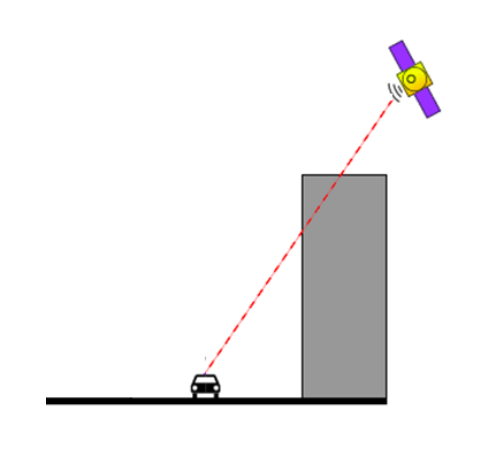
\includegraphics[width=\textwidth]{images/hide.png}
            \caption{遮挡问题}
            \label{fig:hide}
        \end{subfigure}
        \begin{subfigure}[b]{0.48\textwidth}
            \centering
            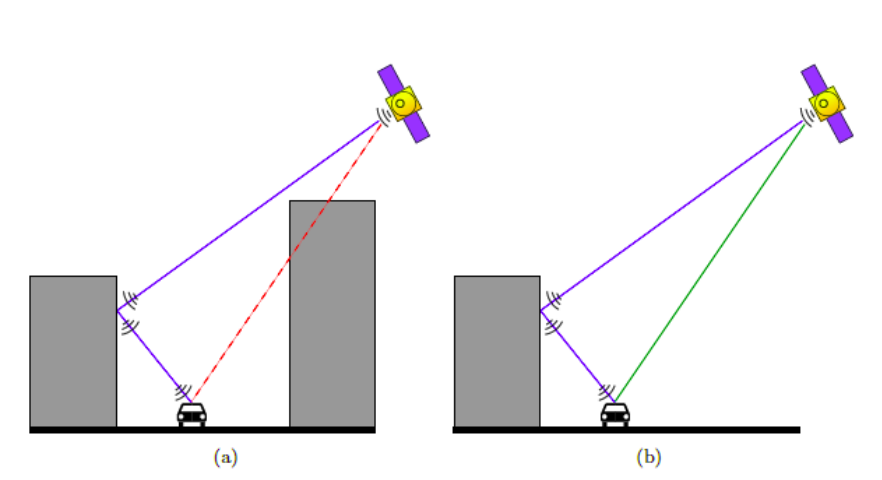
\includegraphics[width=\textwidth]{images/multipath.png}
            \caption{多路径问题}
            \label{fig:multipath}
        \end{subfigure}
        \caption{全球定位系统的问题}
        \label{fig:gps_issues}
    \end{figure}
    \end{itemize}
    \item \textbf{全局视觉观测定位}
            \begin{figure}[H]
                \centering
                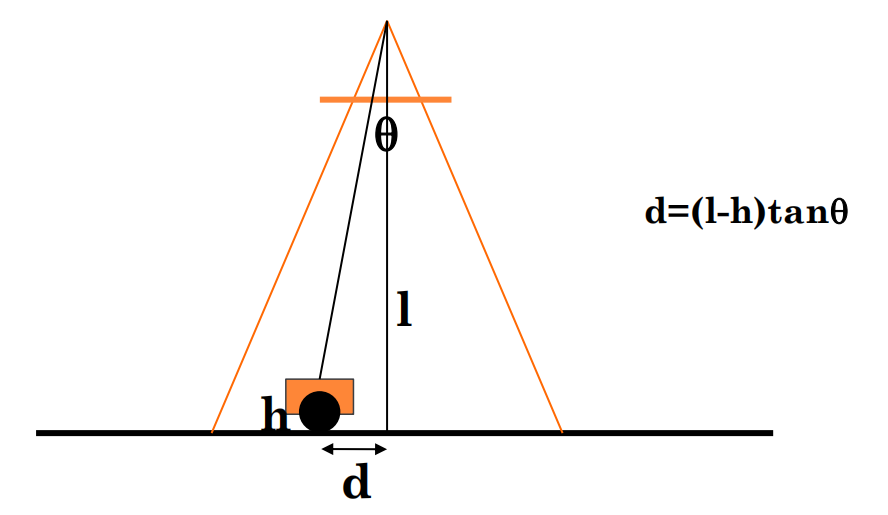
\includegraphics[width=0.5\textwidth]{images/visonlocate.png}
                \caption{视觉定位,如果需要更大的视野,则架设多个相机}
            \end{figure}
    \begin{itemize}
        \item \textbf{基本思想}:搭建一套外部视觉系统,识别机器人,确定其位置
        \item \textbf{应用约束}:
        \begin{itemize}
            \item 摄像头有\textbf{视野范围约束},当环境较大时需要多个摄像头
            \item 机器人上需要有一定的\textbf{标识}方便图像识别定位
        \end{itemize}
    \end{itemize}
    \item \textbf{成本分析}
    \begin{itemize}
        \item 机器人本体实现简单,直接接受定位结果,可降低成本
        \item 外部感知系统成本较高,且感知范围越大,成本越高
    \end{itemize}
\end{enumerate}
\subsection{基于本体感知的定位}
\begin{enumerate}
            \begin{figure}[H]
                \centering
                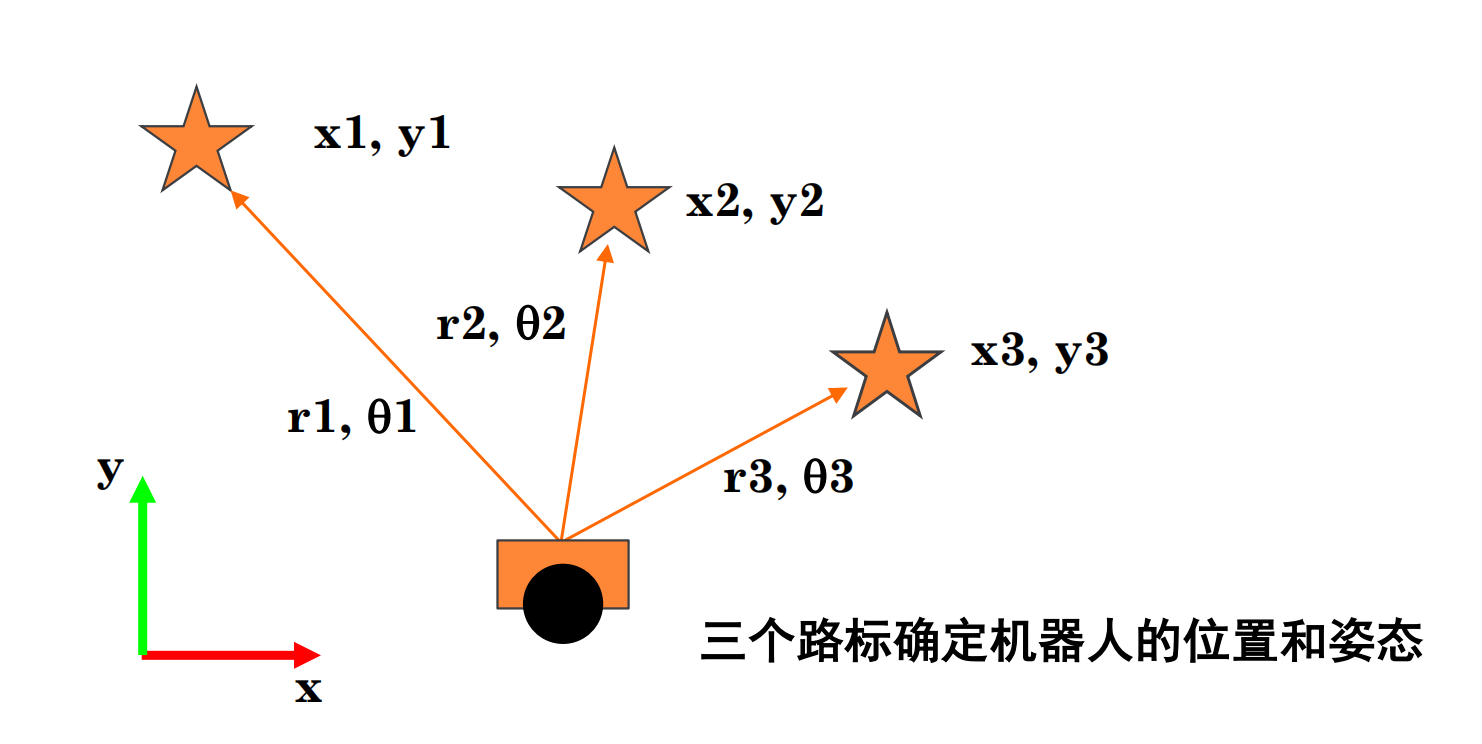
\includegraphics[width=0.5\textwidth]{images/3lubiao.png}
                \caption{三个路标确定机器人的位置和姿态}
            \end{figure}
    \item \textbf{基于空间标识的定位}
        \begin{itemize}
            \item \textbf{基于环境人工标识的定位}:在环境中部署特殊标签,降低成本,确保可靠性
                \begin{itemize}
                    \item 地面二维码
                    \item 激光反射板
                \end{itemize}
            \item \textbf{基于环境自然标识的定位}
        \end{itemize}
    \item \textbf{基于位置识别的定位}
        \begin{itemize}
            \item \textbf{基本思想}:利用本体传感器获得的信息与地图中存储的各个位置上的信息进行匹配,实现位置识别
            \item \textbf{应用约束}:
            \begin{itemize}
                \item 环境的\textbf{动态变化}和不同位置的\textbf{相似性},对位置辨别带来挑
                \item 战为适应环境的动态变化,可以考虑对每个位置存储\textbf{多张图片},但增加存储空间需求
                \item 图像匹配是一个\textbf{耗时}的工作
            \end{itemize}
        \end{itemize}
    \item \textbf{特点}
    \begin{itemize}
        \item 需要\textbf{预先构建地图},地图坐标系在构建地图时确定
        \item 对于大规模环境,路标需具备\textbf{可鉴别性},否则需要正确的数据关联
        \item 存储大规模环境的图片需要较大的\textbf{存储空间}
        \item 对于实际环境中存在路标被破坏/污染、更换、稀疏等风险
    \end{itemize}
\end{enumerate}
\newpage
\subsection*{概统知识回顾}
\hspace{2em}在正式开始对马尔可夫自定位的介绍之前,我们最好回顾一下相关概率论与数理统计的知识基础;本部分是我自己加的\footnote{本节参考自ZJUDancer视觉组内训,https://www.bilibili.com/video/BV1wUmPYCERx/?spm_id_from=333.337.search-card.all.click&vd_source=5deca47094767260f853b759a625a68f},对此感到熟悉的同学可以直接跳过到\hyperref[sec:markov]{控制感知信息融合的的自定位}继续阅读。
    \begin{enumerate}
        \item \textbf{全概率公式}:设事件组 \( {B}_{1},{B}_{2},\ldots ,{B}_{n} \) 满足下列条件
        \begin{enumerate}
            \item \( \mathop{\sum }\limits_{{i = 1}}^{n}{B}_{i} = S \) ;
            \item \( {B}_{1},{B}_{2},\ldots ,{B}_{n} \) 互不相容;
            \item \( P\left( {B}_{i}\right)  > 0,i = 1,2,\ldots n \)
        \end{enumerate}
        则对任意事件 \( A \) ,有 
        $$ P\left( A\right)  = \mathop{\sum }\limits_{{i = 1}}^{n}P\left( {B}_{i}\right) P\left( {A \mid  {B}_{i}}\right) $$

        \item \textbf{贝叶斯公式}:
        \begin{itemize}
            \item 对随机事件 \( \mathrm{A} \) , \( \mathrm{B} \) ,有
            $$ P\left( {B \mid  A}\right)  = \frac{P\left( {AB}\right) }{P\left( A\right) } = \frac{P\left( B\right) P\left( {A \mid  B}\right) }{P\left( A\right) } $$
            \item 对随机事件 \( \mathrm{A},\mathrm{B},\mathrm{C} \) ,若 \( P\left( {A \mid  C}\right)  > 0 \) ,有
            $$ P\left( {B \mid  A,C}\right)  = \frac{P\left( {B \mid  C}\right) P\left( {A \mid  B,C}\right) }{P\left( {A \mid  C}\right) } $$
        \end{itemize}

        \item \textbf{随机变量和与积的期望与方差}:

    设随机变量 $X,Y$ 的均值与方差分别为 $\mu_X,\sigma_X^2$ 与 $\mu_Y,\sigma_Y^2$,协方差为
    $\operatorname{Cov}(X,Y)=\mathbb{E}[(X-\mu_X)(Y-\mu_Y)]$。有如下恒等式:
    
    \begin{enumerate}
      \item \textbf{一般恒等式(不要求独立):}
      \begin{align}
        \mathbb{E}[X+Y] &= \mathbb{E}[X]+\mathbb{E}[Y],\\
        \operatorname{Var}(X+Y) &= \operatorname{Var}(X)+\operatorname{Var}(Y)+2\,\operatorname{Cov}(X,Y),\\
        \mathbb{E}[XY] &= \operatorname{Cov}(X,Y)+\mathbb{E}[X]\mathbb{E}[Y],\\
        \operatorname{Var}(aX+b) &= a^2\,\operatorname{Var}(X)\quad(\text{$a,b$ 常数}),\\
        \operatorname{Cov}(aX+b,\;cY+d) &= ac\,\operatorname{Cov}(X,Y).
      \end{align}
      标准差由方差取平方根得到:$\operatorname{Std}(Z)=\sqrt{\operatorname{Var}(Z)}$。
    
      \item \textbf{独立情形($X \perp\!\!\!\perp Y$)的化简:}
      \[
        \operatorname{Cov}(X,Y)=0,\qquad
        \mathbb{E}[XY]=\mathbb{E}[X]\mathbb{E}[Y]=\mu_X\mu_Y.
      \]
      因而
      \begin{align}
        \operatorname{Var}(X+Y) &= \sigma_X^2+\sigma_Y^2,\\
        \operatorname{Std}(X+Y) &= \sqrt{\sigma_X^2+\sigma_Y^2},\\
        \operatorname{Var}(XY) &= \mathbb{E}[X^2]\mathbb{E}[Y^2]-\big(\mathbb{E}[X]\mathbb{E}[Y]\big)^2 \nonumber\\
          &= (\sigma_X^2+\mu_X^2)(\sigma_Y^2+\mu_Y^2)-\mu_X^2\mu_Y^2 \nonumber\\
          &= \sigma_X^2\sigma_Y^2+\mu_Y^2\sigma_X^2+\mu_X^2\sigma_Y^2,\\
        \operatorname{Std}(XY) &= \sqrt{\sigma_X^2\sigma_Y^2+\mu_Y^2\sigma_X^2+\mu_X^2\sigma_Y^2}.
      \end{align}
    
      \item \textbf{高斯(正态)情形的特殊运算:}
      \begin{itemize}
        \item 若 $X\sim\mathcal{N}(\mu_X,\sigma_X^2)$,$Y\sim\mathcal{N}(\mu_Y,\sigma_Y^2)$ 且独立,则
        \[
          X+Y \sim \mathcal{N}\big(\,\mu_X+\mu_Y,\;\sigma_X^2+\sigma_Y^2\,\big).
        \]
        更一般地,$aX+b \sim \mathcal{N}(a\mu_X+b,\;a^2\sigma_X^2)$。
        \item \textbf{关于积:} 当 $X,Y$ 独立且高斯时,$XY$ 的分布不再是高斯(称为“正态积分布”),
        但其前两阶矩可由上式给出:
        \[
          \mathbb{E}[XY]=\mu_X\mu_Y,\qquad
          \operatorname{Var}(XY)=\sigma_X^2\sigma_Y^2+\mu_Y^2\sigma_X^2+\mu_X^2\sigma_Y^2.
        \]
      \end{itemize}

        \item \textbf{马尔可夫性}:下一时刻的状态只与当前状态有关,与上一时刻状态无关。
        \item \textbf{马尔可夫过程}:具有马尔可夫定性的过程,即:
        $$ P\left( {{S}_{n} = {i}_{n} \mid  {S}_{n - 1} = {i}_{n - 1},\ldots ,{S}_{0} = {i}_{0}}\right)  = P\left( {{S}_{n} = {i}_{n} \mid  {S}_{n - 1} = {i}_{n - 1}}\right) $$
        \item 在机器人定位问题中,还具有如下假设:
            \begin{itemize}
                \item 当前观测可由当前状态完全确定,即状态确定时,观测量与其他变量独立
                \item 当前状态可由上一时刻状态和控制量完全确定,即上一时刻状态和控制量确定时,当前状态与其他变量独立
            \end{itemize}
        \end{enumerate}
        设$t$时刻机器人状态(位置)为$x_t$,观测为$z_t$,控制信息为$u_t$,地图为$m$,则需求出
        $$p(x_t\mid z_{1:t},u_{1:t-1},m)$$
        ,即已知从最初到现在所有的观测信息,最初到上一时刻所有的控制信息以及地图,求机器人位于位姿$x_t$的概率。
        



    \end{enumerate}

\newpage
\subsection{控制感知信息融合的的自定位}\label{sec:markov}
\begin{enumerate}
    \item \textbf{基本概念}:给定环境地图(对环境的已有知识)的条件下,根据机器人的运动控制/里程估计信息和传感器感知数据(当前认知)估计机器人相对于环境地图的坐标。
    \item \textbf{问题分类}:
    \begin{enumerate}
        \item \textbf{位置跟踪(position tracking)}:机器人初始位置已知,需要解决对里程计累积误差的补偿
        \item \textbf{全局定位(global localization)}:机器人初始位置未知
        \item \textbf{绑架问题(kidnapped robot problem)}:机器人在定位良好的条件下突然被移到另一个未被告知的地方\footnote{与全局定位问题的差异在于,当机器人被绑架时,机器人可能已经对自已所在的位置非常确信了},用于检测定位算法发现错误并从错误中恢复的能
    \end{enumerate}
    \item \textbf{简单方法}:根据观测进行定位,没有观测根据里程估计进行航位推算
        \begin{itemize}
            \item \textbf{缺点}:如何融合?
                \begin{itemize}
                    \item 观测存在不确定性,里程估计也存在不确定性,如何\textbf{融合是否观测}
                    \item 观测到多个特征(例如多个交通标志)时,如何\textbf{融合多个观测}进行估
                \end{itemize}
            \item \textbf{解决方案}:
                \begin{itemize}
                    \item 对不确定性进行描述(称为\textbf{置信度}),在\textbf{概率架构}下进行融合
                    \item 用\textbf{方差}表示置信度,方差小表示置信度高
                    \item 控制感知信息融合的自定位就是利用里程估计和观测信息估计\textbf{方差最小}下的机器人位姿
                \end{itemize}
        \end{itemize}
    \item \textbf{概率描述}:定位问题可以定义为\textbf{最优估计问题},最优估计的一个体现是估计的方差很小——用贝叶斯估计器\textbf{是一种最小方差估计器}\\
            我们希望计算:
        \[
        \widehat{\mathbf{X}}^{t} \triangleq \mathbb{E}\left[ \mathbf{X}^{t} \mid \mathbf{Z}^{t}, \mathbf{U}^{t-1}, \mathbf{m} \right]
        \]
        即在给定当前时刻以及历史所有观测$\mathbf{Z}^{t}$、上一时刻以及之前所有控制$\mathbf{U}^{t-1}$,以及地图$\mathbf{m}$后,路径的$\mathrm{x}^t$最优估计。
        {\small\kaishu 
        \begin{enumerate}
        \item \textbf{问题定义}:\\
        记地图为 \( \mathrm{m} \) ,\\
\( t \) 时刻机器人位姿为 \( \mathrm{x}_{t} = {\left( {x}_{t},{y}_{t},{\theta }_{t}\right) }^{T} \) ,\\观测信息为 \( {z}_{t} \) ,\\控制信息为 \( {u}_{t} \)\\路径、观测和控制的历史集合定义:
\( {\mathbf{X}}^{t} = \left\{  {{\mathbf{x}}_{0},{\mathbf{x}}_{1},\ldots ,{\mathbf{x}}_{t}}\right\}  \;{\mathbf{Z}}^{t} = \left\{  {{\mathbf{z}}_{0},{\mathbf{z}}_{1},\ldots ,{\mathbf{z}}_{t}}\right\}  \;{\mathbf{U}}^{t - 1} = \left\{  {{\mathbf{u}}_{0},{\mathbf{u}}_{1},\ldots ,{\mathbf{u}}_{t - 1}}\right\} \)
\\求 \( {\widehat{\mathbf{X}}}^{t} \triangleq  \mathbf{E}\left\lbrack  {{\mathbf{X}}^{t} \mid  {\mathbf{Z}}^{t},{\mathbf{U}}^{t - 1},\mathbf{m}}\right\rbrack \)
        \item \textbf{递推关系推导:}\footnote{我们希望在每个时刻只用上一步的结果来更新,通过该递推关系,我们可以实现概率意义下的自定位}
        
        从联合概率出发,根据乘法公式:
        \[
        p(X,Y) = p(Y \mid X) p(X)
        \]
        可得:
        \[
        p(\mathbf{X}^{t} \mid \mathbf{Z}^{t}, \mathbf{U}^{t-1}, \mathbf{m})
        = p(\mathbf{x}_t \mid \mathbf{X}^{t-1}, \mathbf{Z}^{t}, \mathbf{U}^{t-1}, \mathbf{m})
        \, p(\mathbf{X}^{t-1} \mid \mathbf{Z}^{t}, \mathbf{U}^{t-1}, \mathbf{m})
        \]

        因为 \( \mathbf{X}^{t-1} \) 与之后的观测、控制无关:
        \[
        p(\mathbf{X}^{t-1} \mid \mathbf{Z}^{t}, \mathbf{U}^{t-1}, \mathbf{m})
        = p(\mathbf{X}^{t-1} \mid \mathbf{Z}^{t-1}, \mathbf{U}^{t-2}, \mathbf{m})
        \]
        故:
        \[
        p(\mathbf{X}^{t} \mid \mathbf{Z}^{t}, \mathbf{U}^{t-1}, \mathbf{m})
        = p(\mathbf{x}_t \mid \mathbf{X}^{t-1}, \mathbf{Z}^{t}, \mathbf{U}^{t-1}, \mathbf{m})
        \, p(\mathbf{X}^{t-1} \mid \mathbf{Z}^{t-1}, \mathbf{U}^{t-2}, \mathbf{m})
        \]
        
        \item \textbf{引入贝叶斯公式:}
        对等号右端第一项应用贝叶斯公式,得
$$
p(\mathbf{x}_t \mid \mathbf{X}^{t-1}, \mathbf{Z}^{t}, \mathbf{U}^{t-1}, \mathbf{m})
= \frac{
  p(\mathbf{z}_t \mid  \mathbf{X}^{t-1}, \mathbf{Z}^{t-1}, \mathbf{U}^{t-1}, \mathbf{m})
  \;
  p(\mathbf{x}_t \mid \mathbf{X}^{t-1}, \mathbf{Z}^{t-1}, \mathbf{U}^{t-1}, \mathbf{m})
}{
  p(\mathbf{z}_t \mid \mathbf{X}^{t-1}, \mathbf{Z}^{t-1}, \mathbf{U}^{t-1}, \mathbf{m})
}
$$
其中分母
$$
p(\mathbf{z}_t \mid \mathbf{X}^{t-1}, \mathbf{Z}^{t-1}, \mathbf{U}^{t-1}, \mathbf{m})
= \int 
  p(\mathbf{z}_t \mid \mathbf{x}_t, \mathbf{X}^{t-1}, \mathbf{Z}^{t-1}, \mathbf{U}^{t-1}, \mathbf{m})
  \;
  p(\mathbf{x}_t \mid \mathbf{X}^{t-1}, \mathbf{Z}^{t-1}, \mathbf{U}^{t-1}, \mathbf{m})
  \, d\mathbf{x}_t
$$
仅依赖于历史量 $\mathbf{X}^{t-1}, \mathbf{Z}^{t-1}, \mathbf{U}^{t-1}, \mathbf{m}$,与当前状态 $\mathbf{x}_t$ 无关;若被积函数 $f(x \mid c)$ 的条件 $c$ 中不包含积分变量 $x$,则积分 $\int f(x \mid c) \, dx$ 只依赖于 $c$,对 $x$ 而言是常数。故分母可作为常数,记为归一化因子 $\eta$,即
$$
\eta = \frac{1}{
  p(\mathbf{z}_t \mid \mathbf{X}^{t-1}, \mathbf{Z}^{t-1}, \mathbf{U}^{t-1}, \mathbf{m})
}
= \left[
  \int 
  p(\mathbf{z}_t \mid \mathbf{x}_t, \mathbf{X}^{t-1}, \mathbf{Z}^{t-1}, \mathbf{U}^{t-1}, \mathbf{m})
  \;
  p(\mathbf{x}_t \mid \mathbf{X}^{t-1}, \mathbf{Z}^{t-1}, \mathbf{U}^{t-1}, \mathbf{m})
  \, d\mathbf{x}_t
\right]^{-1}
$$
从而
        \[
        p(\mathbf{X}^{t} \mid \mathbf{Z}^{t}, \mathbf{U}^{t-1}, \mathbf{m})
        = \eta \, p(\mathbf{z}_t \mid \mathbf{X}^{t}, \mathbf{Z}^{t-1}, \mathbf{U}^{t-1}, \mathbf{m})
        \, p(\mathbf{x}_t \mid \mathbf{X}^{t-1}, \mathbf{Z}^{t-1}, \mathbf{U}^{t-1}, \mathbf{m})
        \, p(\mathbf{X}^{t-1} \mid \mathbf{Z}^{t-1}, \mathbf{U}^{t-2}, \mathbf{m})
        \]
        
        \item \textbf{根据马尔可夫假设(系统独立性)简化:}
        \begin{enumerate}
            \item 当前状态仅依赖于上一时刻状态与控制量:
            \[
            p(\mathbf{x}_t \mid \mathbf{X}^{t-1}, \mathbf{Z}^{t-1}, \mathbf{U}^{t-1}, \mathbf{m})
            = p(\mathbf{x}_t \mid \mathbf{x}_{t-1}, \mathbf{u}_{t-1}, \mathbf{m})
            \]
            \item 当前观测仅依赖于当前状态:
            \[
            p(\mathbf{z}_t \mid \mathbf{X}^{t}, \mathbf{Z}^{t-1}, \mathbf{U}^{t-1}, \mathbf{m})
            = p(\mathbf{z}_t \mid \mathbf{x}_t, \mathbf{m})
            \]
        \end{enumerate}
        
        将上述代入后,得到最终递推形式:
        \[
        \boxed{
        p(\mathbf{X}^{t} \mid \mathbf{Z}^{t}, \mathbf{U}^{t-1}, \mathbf{m})
        = \eta \, p(\mathbf{z}_t \mid \mathbf{x}_t, \mathbf{m})
        \, p(\mathbf{x}_t \mid \mathbf{x}_{t-1}, \mathbf{u}_{t-1}, \mathbf{m})
        \, p(\mathbf{X}^{t-1} \mid \mathbf{Z}^{t-1}, \mathbf{U}^{t-2}, \mathbf{m})
        }
        \]
        分别代表:\\
        - \( p(\mathbf{X}^{t} \mid \mathbf{Z}^{t}, \mathbf{U}^{t-1}, \mathbf{m}) \):t时刻的后验分布\\
        - \( p(\mathbf{z}_t \mid \mathbf{x}_t, \mathbf{m}) \):观测模型\\
        - \( p(\mathbf{x}_t \mid \mathbf{x}_{t-1}, \mathbf{u}_{t-1}, \mathbf{m}) \):运动模型  \\
        - \( p(\mathbf{X}^{t-1} \mid \mathbf{Z}^{t-1}, \mathbf{U}^{t-2}, \mathbf{m}) \):t-1时刻的后验分布
        
        
        \item \textbf{状态量化形式:}
        实际应用中,我们通常只关心当前位姿的后验,而非整条路径:
        \[
        \mathbf{x}_t = \mathbb{E}\left[\mathbf{x}_t \mid \mathbf{Z}^{t}, \mathbf{U}^{t-1}, \mathbf{m}\right]
        \]
        对应概率递推形式为:
        \end{enumerate}
        \[
        \underbrace{p(\mathbf{x}_t \mid \mathbf{Z}^{t}, \mathbf{U}^{t-1}, \mathbf{m})}_{\text{t时刻位姿}}
        = \eta \;
        \underbrace{p(\mathbf{z}_t \mid \mathbf{x}_t, \mathbf{m})}_{\text{观测模型}} \;
        \int 
        \underbrace {p(\mathbf{x}_t \mid \mathbf{x}_{t-1}, \mathbf{u}_{t-1}, \mathbf{m})
        }_{\text{运动模型}}
        \underbrace{
          \, p(\mathbf{x}_{t-1} \mid \mathbf{Z}^{t-1}, \mathbf{U}^{t-2}, \mathbf{m})
        }_{\text{t-1时刻位姿}}
        \, d\mathbf{x}_{t-1} \]
        }
    \end{enumerate}

该公式被称为\textbf{实时自定位贝叶斯递推公式}。
            \begin{figure}[H]
                \centering
                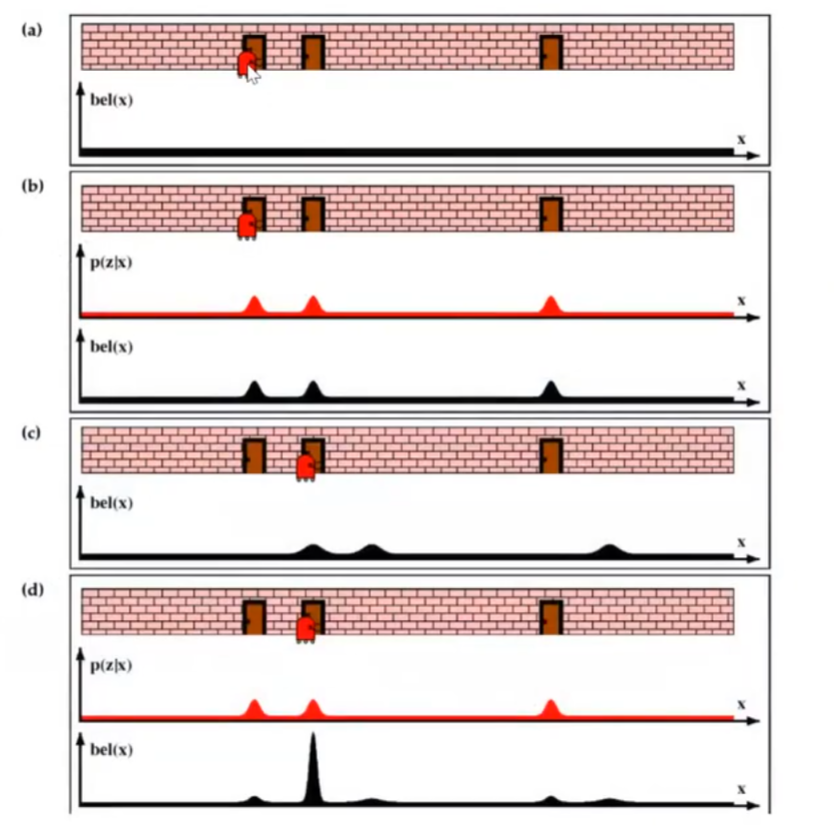
\includegraphics[width=0.5\textwidth]{images/markov_example.png}
                \caption{马尔可夫自定位流程}
            \end{figure}
            {\small\kaishu 如上图所示,我们抽象出一个一维运动的例子,用黑色函数代表运动模型得到的概率分布,红色函数代表观测模型得到的概率分布,我们机器人的自定位实际上是如下的过程:
            \begin{itemize}
                \item 先用运动模型:机器人初始化,可能在地图上任何一个位置出现,此时其运动模型是均匀分布的;
                \item 再用观测模型:随后在图(b)机器人开始观测,发现有一个门,那机器人判断自己在三扇门出现的概率会更高,其他地方概率会更低,修正了运动模型
                \item 机器人向前运动,如图(c),继续用运动模型,对位姿进行预测,机器人预测自身的位置肯定整体向右移动了
                \item 再用观测模型:随后在图(d)机器人开始观测,发现还有一个门,那机器人判断自己出现在第二扇门出现的概率会更高,据此再次修正了运动模型
            \end{itemize}}
            
\subsection{马尔可夫定位中的运动模型}
        在上一节,我们得到了实时自定位贝叶斯递推公式
        \[
        p(\mathbf{x}_t \mid \mathbf{Z}^{t}, \mathbf{U}^{t-1}, \mathbf{m})
        = \eta \, p(\mathbf{z}_t \mid \mathbf{x}_t, \mathbf{m})
        \int \textcolor{red}{p(\mathbf{x}_t \mid \mathbf{x}_{t-1}, \mathbf{u}_{t-1}, \mathbf{m})}
        \, p(\mathbf{x}_{t-1} \mid \mathbf{Z}^{t-1}, \mathbf{U}^{t-2}, \mathbf{m})
        \, d\mathbf{x}_{t-1}
        \]
        对红色项(运动模型),利用贝叶斯规则
        $$\textcolor{red}{p(\mathbf{x}_t \mid \mathbf{x}_{t-1}, \mathbf{u}_{t-1}, \mathbf{m})}=\eta     \textcolor{blue}{p(\mathrm{m}|\mathrm{x}_t,\mathrm{x}_{t-1},\mathrm{u}_{t-1})}\textcolor{orange}{p(\mathrm{x}_t|\mathrm{x}_{t-1},\mathrm{u}_{t-1})}$$
        \begin{itemize}
            \item 橙色项:给定上一时刻位姿$x_{t-1}$和控制指令$u_{t-1}$,计算当前位姿$x_{t}$的概率分布
            \item 蓝色项:在控制指令$u_{t-1}$下机器人从$x_{t-1}$移动到$x_{t}$,在这样条件下地图$m$的可能性\footnote{如果路径或者$x_t$与环境障碍物碰撞,则获得地图$m$的可能性低。通过路径验证地图存在的可能性,实现地图条件下当前位姿估计的验证}
            \begin{figure}[H]
                \centering
                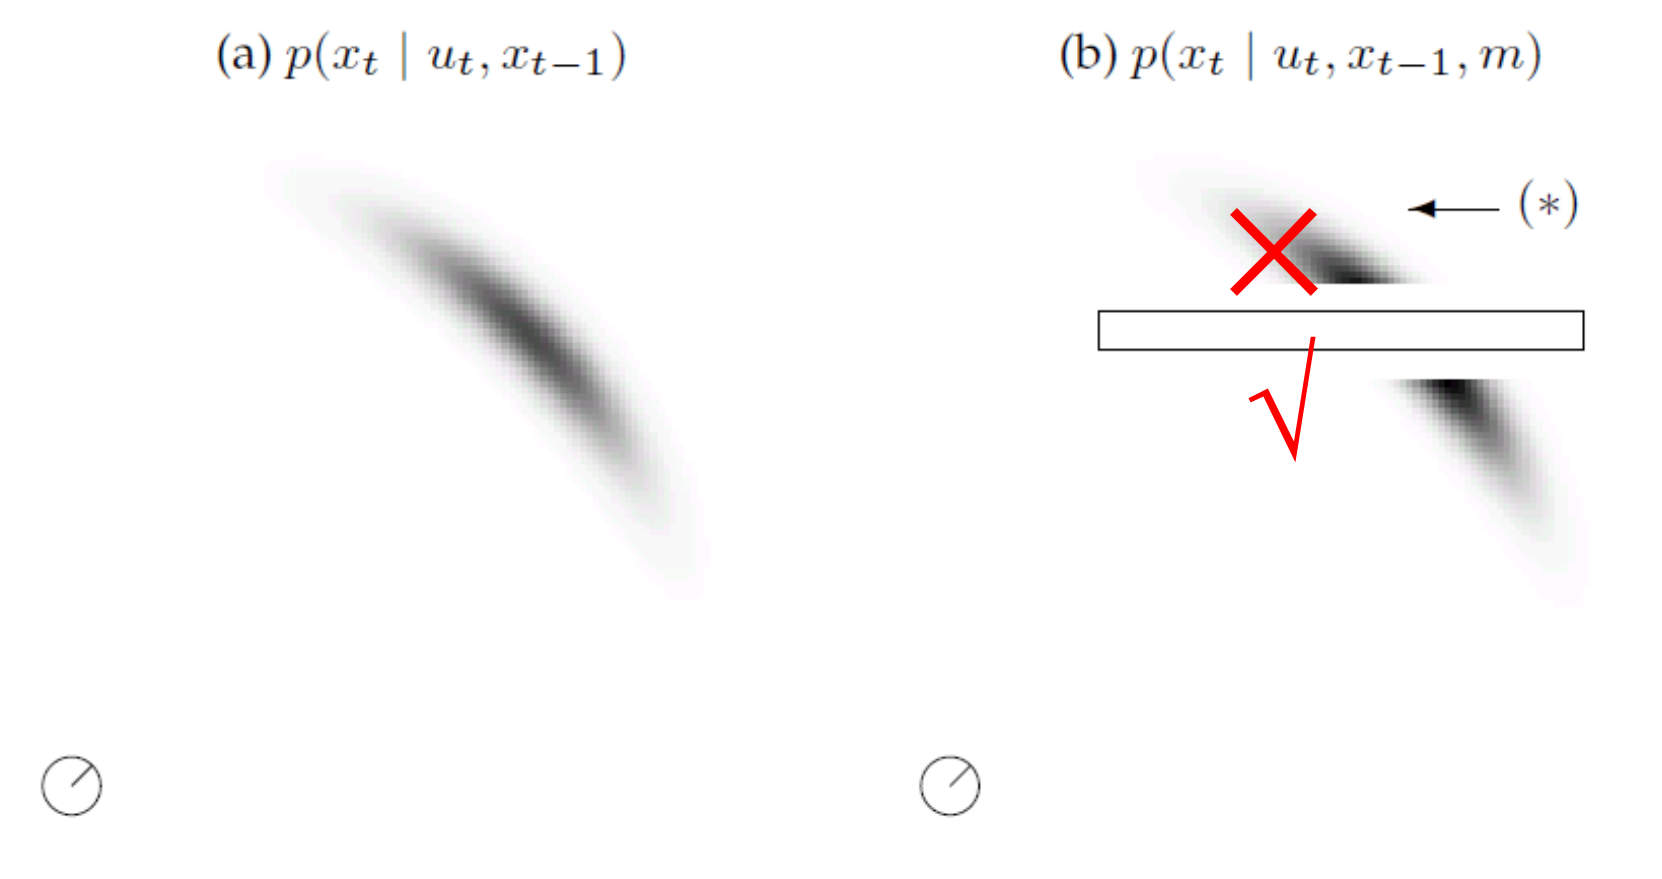
\includegraphics[width=0.3\textwidth]{images/map.png}
                \caption{考虑地图的运动模型}
            \end{figure}
            {\small\kaishu 
            $$ \mathbf{p}\left( {{\mathrm{x}}_{t} \mid  {\mathrm{x}}_{t - 1},{\mathbf{u}}_{t - 1},\mathbf{m}}\right)  = \mathbf{m}\left( {\mathbf{m} \mid  {\mathrm{x}}_{t},{\mathrm{x}}_{t - 1},{\mathbf{u}}_{t - 1}}\right) \mathbf{p}\left( {{\mathrm{x}}_{t} \mid  {\mathrm{x}}_{t - 1},{\mathbf{u}}_{t - 1}}\right)$$
            地图分为可通行和不可通行\\
            本项作用: 基于地图降低运动模型的不确定性\\
            问题:需要融合两次位姿之间路径不被占用的可能性和机器人根据控制跟随该路径的可能性,计算非常复杂,难以计算闭式解\\
            实际应用时,可以
            $$ p\left( {{\mathbf{x}}_{t} \mid  {\mathbf{x}}_{t - 1},{\mathbf{u}}_{t - 1},\mathbf{m}}\right)  \approx  p\left( {{\mathbf{x}}_{t} \mid  {\mathbf{x}}_{t - 1},{\mathbf{u}}_{t - 1}}\right) $$
            $$ p\left( {{\mathbf{x}}_{t} \mid  {\mathbf{x}}_{t - 1},{\mathbf{u}}_{t - 1},\mathbf{m}}\right)  \approx  {\eta p}\left( {{\mathbf{x}}_{t} \mid  {\mathbf{x}}_{t - 1},{\mathbf{u}}_{t - 1}}\right) p\left( {{\mathbf{x}}_{t} \mid  \mathbf{m}}\right) $$
            }
        \end{itemize}
        显然,当采用不同的控制指令即不同的$u$时,概率运动模型也是不同的。接下来,我们分别从
        \begin{itemize}
            \item \textbf{里程计运动模型}:$u_{t-1}$是\textbf{里程估计数据},回顾其航位推算计算公式:
            $$\begin{cases}x_t=x_{t-1}+\Delta d\cos(\theta_{t-1}+\Delta\theta)\\y_t=y_{t-1}+\Delta d\sin(\theta_{t-1}+\Delta\theta)\\\theta_t=\theta_{t-1}+\Delta\theta\end{cases}$$
            \item \textbf{速度运动模型}:$u_{t-1}$是\textbf{控制机器人运动的指令},回顾其航位推算计算公式:
            $$\left.\left(\begin{array}{c}x'\\y'\\\theta'\end{array}\right.\right)=\left(\begin{array}{c}x-\frac{\nu}{\omega}\sin(\theta)+\frac{\nu}{\omega}\sin(\theta+\omega\Delta t)\\y+\frac{\nu}{\omega}\cos(\theta)-\frac{\nu}{\omega}\cos(\theta+\omega\Delta t)\\\theta+\omega\Delta t\end{array}\right)$$
        \end{itemize}

\begin{enumerate}
    \item \textbf{里程计运动模型}\\
    我们的最终目的是计算出$$p(\mathrm{x}_t|\mathrm{x}_{t-1},\mathrm{u}_{t-1})$$
    在里程计运动模型中,我们认为$\mathrm{u}_{t-1}$是$\boldsymbol{\delta} = (\delta_{rot1}, \delta_{trans}, \delta_{rot2})^T$
                \begin{figure}[H]
                \centering
                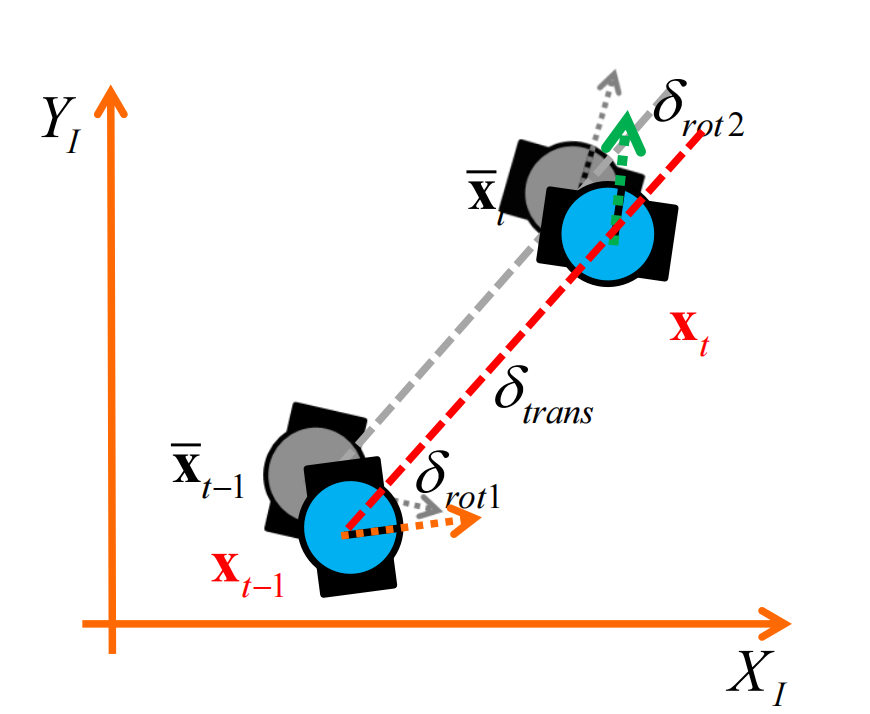
\includegraphics[width=0.3\textwidth]{images/licheng_model1.png}
                \caption{里程计运动模型变量假设}
            \end{figure}
    \begin{enumerate}
        \item \textbf{理想(无噪声)状态下的航位变化}\\
        我们假设机器人先旋转$\delta_{rot1}$、平移$\delta_{trans}$、再旋转$\delta_{rot2}$,将运动变化量        
        
        $$\boldsymbol{\delta} = (\delta_{rot1}, \delta_{trans}, \delta_{rot2})^T$$
        
        叠加到$\mathbf{x}_{t-1}=(x,y,\theta)^T\text{得到}\mathbf{x}_t=(x',y',\theta')^T$
        $$\begin{pmatrix}x'\\y'\\\theta'\end{pmatrix}=\begin{pmatrix}x+\delta_{trans}\cos(\theta+\delta_{rot1})\\y+\delta_{trans}\sin(\theta+\delta_{rot1})\\\theta+\delta_{rot1}+\delta_{rot2}\end{pmatrix}$$

        \item \textbf{不理想(有噪声)状态下的航位变化}\\
        显然,实际测量中是带有各种原因导致的误差的,这里的$$\boldsymbol{\delta} = (\delta_{rot1}, \delta_{trans}, \delta_{rot2})^T$$
        考虑误差后,用头尖尖表示真实值,用波浪线代表误差,不戴帽子是测量值,实际上可以写作
        $$\boldsymbol{\delta} = ({\widehat{\delta }}_{rot1},{\widehat{\delta }}_{trans}, {\widehat{\delta }}_{rot2})^T$$
        根据\textbf{“真实值 = 测量值 - 误差”},其中
        $${\widehat{\delta }}_{rot1} = {\delta }_{rot1} - {\widetilde{\delta }}_{rot1}$$
        $${\widehat{\delta }}_{trans} = {\delta }_{trans} - {\widetilde{\delta }}_{trans}$$
        $${\widehat{\delta }}_{rot2} = {\delta }_{rot2} - {\widetilde{\delta }}_{rot2} $$
        那么实际的航位变化是
        \( \left( \begin{array}{l} {x}^{\prime } \\  {y}^{\prime } \\  {\theta }^{\prime } \end{array}\right)  = \left( \begin{matrix} x + {\widehat{\delta }}_{\text{trans }}\cos \left( {\theta  + {\widehat{\delta }}_{rot1}}\right) \\  y + {\widehat{\delta }}_{\text{trans }}\sin \left( {\theta  + {\widehat{\delta }}_{rot1}}\right) \\  \theta  + {\widehat{\delta }}_{rot1} + {\widehat{\delta }}_{rot2} \end{matrix}\right) \)
                \item \textbf{闭式求解运动模型}\\
            {\small\kaishu \textcolor{red}{闭式求解是看想要控制量的误差$\widetilde{\mathbf{u}}_{t-1}$:
            \begin{enumerate}
                \item 已知上一时刻的位姿$\mathbf{x}_{t-1}$、控制量$\mathbf{u}_{t-1}$
                \item 假设一个接下来可能到达的候选位姿$\mathbf{x}_t$
                \item 然后用逆模型(位姿→控制)计算,从$\mathbf{x}_{t-1}$到$\mathbf{x}_{t}$,需要执行什么控制$\widehat{\mathbf{u}}_{t-1}$?
                \item 比较$\widehat{\mathbf{u}}_{t-1}$与$\mathbf{u}_{t-1}$,误差越大,越不可能
            \end{enumerate}
            }}
            \begin{enumerate}
                \item \textbf{测量控制值}:将里程计数据 \( {\mathbf\mathbf{u}}_{t - 1} \) 表示为 \( \mathbf{\delta } = {\left( {\delta }_{rot1},{\delta }_{trans},{\delta }_{rot2}\right) }^{T} \) ,作为测量控制值
                \item \textbf{真实控制值}:根据 \( {\mathbf{x}}_{t - 1},{\mathbf{x}}_{t} \) 计算机器人的实际运动变化量 \( \widehat{\mathbf{\delta }} = {\left( {\widehat{\delta }}_{rot1},{\widehat{\delta }}_{trans},{\widehat{\delta }}_{rot2}\right) }^{T} \) ,作为真实控制值           
                \item \textbf{估计分布}:根据真实值与测量值之间误差 \( \widetilde{\delta } = \delta  - \widehat{\delta } \) 的分布估计 \( {\mathbf{x}}_{t} \) 的分布
                
                $$ \boxed{p\left( {{\mathbf{x}}_{t} \mid  {\mathbf{x}}_{t - 1},{\mathbf{u}}_{t - 1}}\right)  = p\left( {\widetilde{\delta }}_{rot1}\right)  \cdot  p\left( {\widetilde{\delta }}_{trans}\right)  \cdot  p\left( {\widetilde{\delta }}_{rot2}\right)} $$
            \end{enumerate}

         \item \textbf{误差的概率分布}\\
         真实值与测量值之间的误差应服从该分布“误差越小,概率越高;误差越大,概率越低”,我们可以设定误差为均值为0的高斯分布
            \begin{figure}[H]
                \centering
                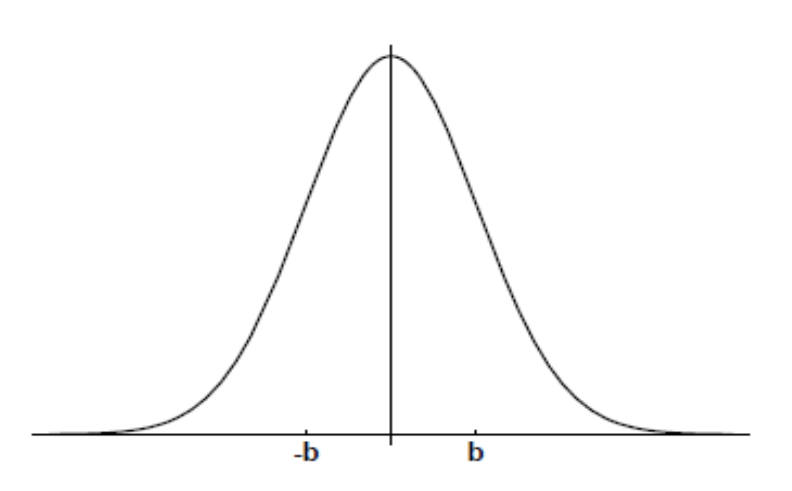
\includegraphics[width=0.3\textwidth]{images/guass.png}
                \caption{设定为高斯分布的误差}
            \end{figure}
            $$ p( \widehat{\delta }_{rot1})  = N\left( {{\widetilde{\delta }}_{{rot}1};0,{\alpha }_{1}\left| {\delta }_{{rot}1}\right|  + {\alpha }_{2}\left| {\delta }_{trans}\right| }\right) $$
            $$ p\left( {\widetilde{\mathbf{\delta }}}_{\text{trans }}\right)  = N\left( {{\widetilde{\mathbf{\delta }}}_{\text{trans }};0,{\alpha }_{3}\left| {\mathbf{\delta }}_{\text{trans }}\right|  + {\alpha }_{4}\left| {{\mathbf{\delta }}_{\text{rot1 }} + {\mathbf{\delta }}_{\text{rot2 }}}\right| }\right) $$
            $$ p\left( {\widetilde{\delta }}_{rot2}\right)  = N\left( {{\widetilde{\delta }}_{rot2};0,{\alpha }_{1}\left| {\delta }_{rot2}\right|  + {\alpha }_{2}\left| {\delta }_{trans}\right| }\right) $$
                        {\small\kaishu 
            显然,平移造成的误差和旋转造成的误差不可能对所有机器人都是一比一的,因此我们设定一些参数$\alpha_i$来作为权重;对于旋转误差例如${\widetilde{\delta }}_{{rot}1}$,其误差组成包括旋转造成的旋转误差和平移造成的旋转误差两部分;平移误差同理。
            }

        \item \textbf{随机采样求解运动模型}\\
            {\small\kaishu \textcolor{red}{随机采样求解是看加上随机误差的控制量$\widetilde{\mathbf{u}}_{t-1}$下$ \mathbf{x}_t $更有可能落到哪里:
            \begin{enumerate}
                \item 已知上一时刻的测量控制值$\mathbf{u}_{t-1}$ ,
                \item 假设一个噪声$\widetilde{\mathbf{u}}_{t-1}$,得到真实控制值$\widehat{\mathbf{u}}_{t-1}$
                \item 然后用正模型(控制→位姿)计算,从$\mathbf{x}_{t-1}$执行控制$\widehat{\mathbf{u}}_{t-1}$,会到达什么$\mathbf{x}_{t}$?
                \item 重复若干次 → 得到若干个 $ \mathbf{x}_t $ 样本,落的点多的地方就是高概率区
            \end{enumerate}
            }}
            \begin{enumerate}
                \item \textbf{计算误差}:在噪声的高斯分布中随机采样\footnote{sample是一个计算机函数,调用时需传参均值和方差。均值对于误差而言就是0,我们先根据里程计的读数$\delta$和$\alpha$参数,计算出误差分布的方差$\sigma^2$;用采样函数,从一个均值为0、方差为我们刚刚计算出的$\sigma^2$的正态分布中,随机抽取一个具体的误差值$\widetilde{\delta }$。}
                $${\widetilde{\delta }}_{rot1} = {sample}\left( {{\alpha }_{1}\left| {\delta }_{rot1}\right|  + {\alpha }_{2}\left| {\delta }_{trans}\right| }\right) ,{\widetilde{\delta }}_{trans} = \cdots ,{\widetilde{\delta }}_{rot2} = ... $$
                基于采样得到的噪声和测量得到的里程计值,构建机器人实际执行
                的控制指令\footnote{其实是基于采样得到的噪声和测量得到的里程计值,构建对机器人实际发生的物理运动$\widehat{\delta }$的一次随机估计}
                $$ {\widehat{\delta }}_{rot1} = {\delta }_{rot1} - {\widetilde{\delta }}_{rot1},{\widehat{\delta }}_{trans} = {\delta }_{trans} - {\widetilde{\delta }}_{trans},{\widehat{\delta }}_{rot2} = {\delta }_{rot2} - {\widetilde{\delta }}_{rot2} $$    
                \item \textbf{计算$\mathrm{x}_t$}:利用前述里程运动叠加模型计算$\mathrm{x}_t$
                \item \textbf{重复计算}:重复上述过程,所得 \( {\mathbf{x}}_{t} \) 点集合构成对 \( p\left( {{\mathbf{x}}_{t} \mid  {\mathbf{x}}_{t - 1},{\mathbf{u}}_{t - 1}}\right) \) 的描述
            \end{enumerate}
                \begin{figure}[H]
                \centering
                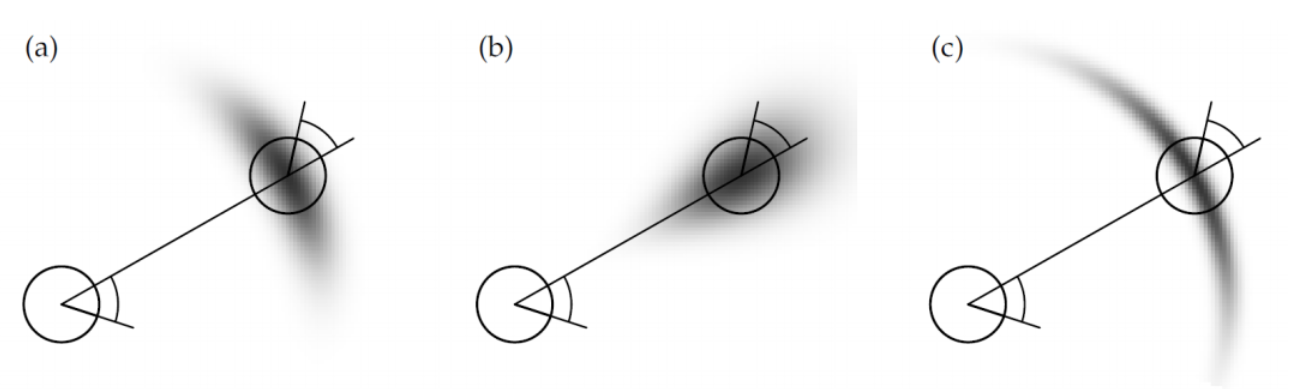
\includegraphics[width=0.6\textwidth]{images/alpha0.png}
                \caption{不同$\alpha_i$参数下通过\textbf{闭式求解}得到的$p(\mathrm{x}_t,\mathrm{x}_{t-1},\mathrm{u}_{t-1})$;对比发现,(a)图对旋转和平移误差的权重相对均一,图(b)平移误差权重更大,图(c)旋转误差权重更大}
                \end{figure}
                \begin{figure}[H]
                \centering
                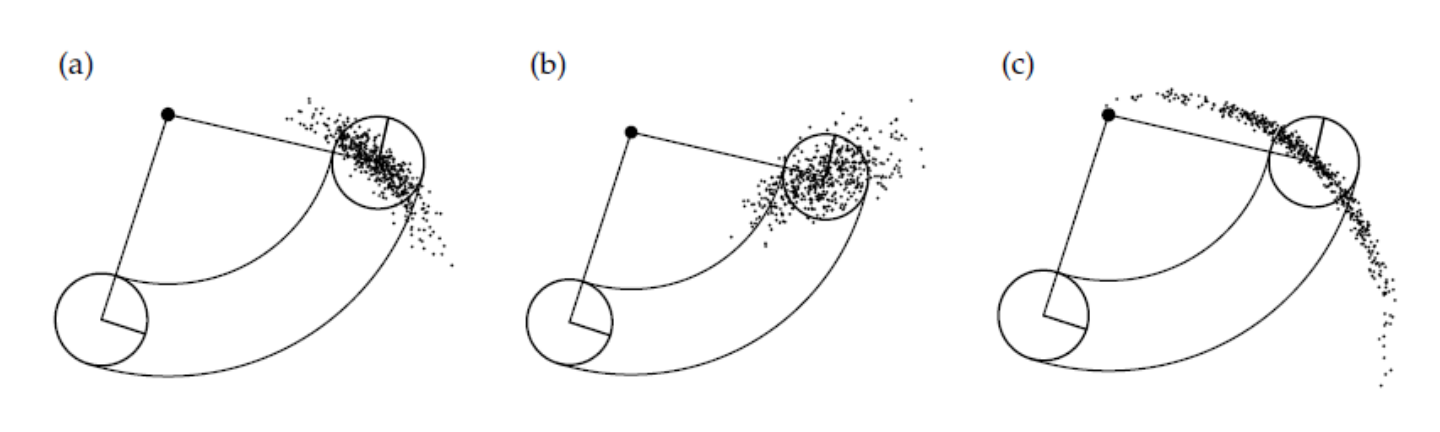
\includegraphics[width=0.6\textwidth]{images/alpha.png}
                \caption{不同$\alpha_i$参数下通过\textbf{随机采样求解}得到的$p(\mathrm{x}_t,\mathrm{x}_{t-1},\mathrm{u}_{t-1})$,每个子图含500个样本;对比发现,(a)图对旋转和平移误差的权重相对均一,图(b)平移误差权重更大,图(c)旋转误差权重更大}
                \end{figure}
        
\end{enumerate}
    \item \textbf{速度运动模型}\\
    我们的最终目的是计算出$$p(\mathrm{x}_t|\mathrm{x}_{t-1},\mathrm{u}_{t-1})$$
    在速度运动模型中,我们认为$\mathrm{u}_{t-1}$是$(v,\omega)$
    \begin{enumerate}
        \item \textbf{理想(无噪声)状态下的航位变化}\\
        $$\begin{pmatrix} x' \\ y' \\ \theta' \end{pmatrix} = \begin{pmatrix} x - \frac{v}{\omega} \sin(\theta) + \frac{v}{\omega} \sin(\theta + \omega \Delta t) \\ y - \frac{v}{\omega} \cos(\theta) + \frac{v}{\omega} \cos(\theta + \omega \Delta t) \\ \theta + \omega \Delta t \end{pmatrix}$$

        \item \textbf{不理想(有噪声)状态下的航位变化}\\
        根据\textbf{“真实控制值 = 指令测量值 + 误差”},其中
        $$\widehat{v}=v+\widetilde{v}$$
        $$\widehat{\omega}=\omega+\widetilde{\omega}$$
        此外,我们考虑圆弧运动假设引起了退化问题(状态量三维,控制量二维)\footnote{实际噪声下,位姿变化可能不完美符合圆弧(比如小方向偏差)},会导致应用贝叶斯估计状态中逆向求解时发生分歧,为此假设机器人到达末位姿后执行转动$\widehat{\gamma}$
        \vspace{1em}
        那么实际的航位变化是
        $$\begin{pmatrix}x'\\y'\\\theta'\end{pmatrix}=\begin{pmatrix}x-\frac{\widehat{v}}{\widehat{\omega}}sin(\theta)+\frac{\widehat{v}}{\widehat{\omega}}sin(\theta+\widehat{\omega}\Delta t)\\y-\frac{\widehat{v}}{\widehat{\omega}}cos(\theta)+\frac{\widehat{v}}{\widehat{\omega}}cos(\theta+\widehat{\omega}\Delta t)\\\theta+\widehat{\omega}\Delta t+\widehat{\gamma}\Delta t\end{pmatrix}$$
        
        \item \textbf{闭式求解运动模型}
        \begin{enumerate}
            \item 根据所评估状态 $\mathbf{x}_t$ 和当前前状态 $\mathbf{x}_{t-1}$ 计算无噪声模型下的实际控制指令$\widehat{\mathbf{u}}_{t-1} = (\widehat{v}, \widehat{\omega}, \widehat{\gamma})$ 
            \item 根据实际控制指令 $\widehat{\mathbf{u}}_{t-1}$ 和发送控制指令 $\mathbf{u}_{t-1}$ 之间误差分布估计 $\mathbf{x}_t$ 的分布
            $$p(\mathbf{x}_t | \mathbf{x}_{t-1}, \mathbf{u}_{t-1}) = \varepsilon_{b_{\widetilde{v}}}(\widetilde{v}) \cdot \varepsilon_{b_{\widetilde{\omega}}}(\widetilde{\omega}) \cdot \varepsilon_{b_{\widetilde{\gamma}}}(\widetilde{\gamma})$$
            $$\widetilde{v} = \widehat{v} - v$$
            $$ \widetilde{\omega} = \widehat{\omega} - \omega$$
            $$ \widetilde{\gamma} = \widehat{\gamma}$$
        \end{enumerate}

        \item \textbf{误差的概率分布}\\
         误差/噪声一般可以建模为均值为0,标准偏差为b的高斯分布或者三角分布
            \begin{figure}[H]
                \centering
                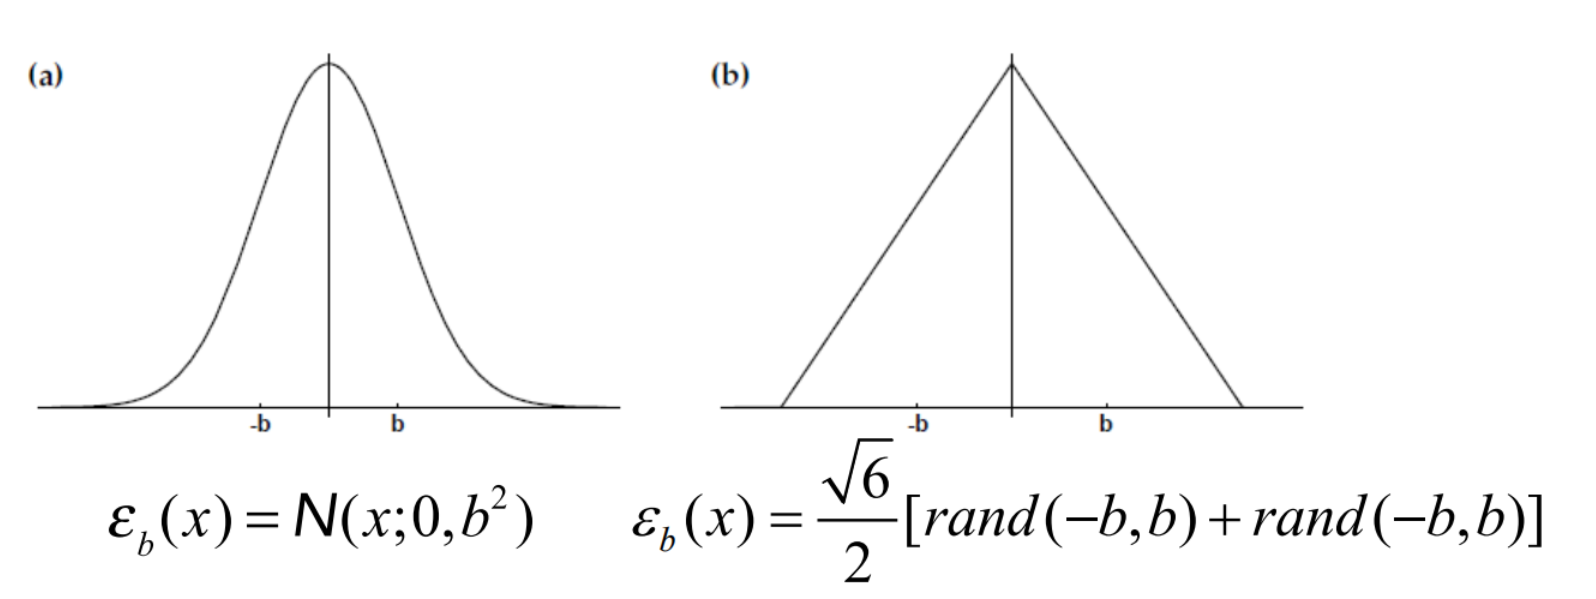
\includegraphics[width=0.3\textwidth]{images/error2.png}
                \caption{设定为高斯分布/三角分布的误差}
            \end{figure}
            可以设:
            $$b_{\widetilde{v}} = \alpha_{1}|v| + \alpha_{2}|\omega|$$
            $$ b_{\widetilde{\omega}} = \alpha_{3}|v| + \alpha_{4}|\omega|$$
            $$b_{\widetilde{\gamma}} = \alpha_{5}|v| + \alpha_{6}|\omega|$$
            
        \item \textbf{随机求解运动模型}
        \begin{enumerate}
            \item 将噪声建模为高斯分布,根据噪声的高斯分布随机采样噪声
            $$\widetilde{v} = \mathrm{sample}(\alpha_1 |v| + \alpha_2 |\omega|)$$
            $$\widetilde{\omega} = \mathrm{sample}(\alpha_3 |v| + \alpha_4 |\omega|)$$
            $$\widetilde{\gamma} = \mathrm{sample}(\alpha_5 |v| + \alpha_6 |\omega|)$$
            \item 基于采样得到的噪声和发送的控制指令,构建机器人实际执行控制指令
            $$\widehat{v} = v + \widetilde{v}$$
            $$\widehat{\omega} = \omega + \widetilde{\omega}$$
            $$\widehat{\gamma} = \widetilde{\gamma}$$
            \item 利用前述正向运动模型计算 $\mathbf{x}_t$
            \item 重复上述过程,所得 $\mathbf{x}_t$ 点集合构成为对 $\mathbf{x}_t$ 的概率分布描述
        \end{enumerate}
\end{enumerate}
\end{enumerate}

        
\vspace{2em}
\textbf{仅用运动模型存在问题}:\\
\textcolor{red}{如果只考虑运动模型进行位姿估计,其不确定性(方差)会不断地无上限增大}
                \begin{figure}[H]
                    \centering
                    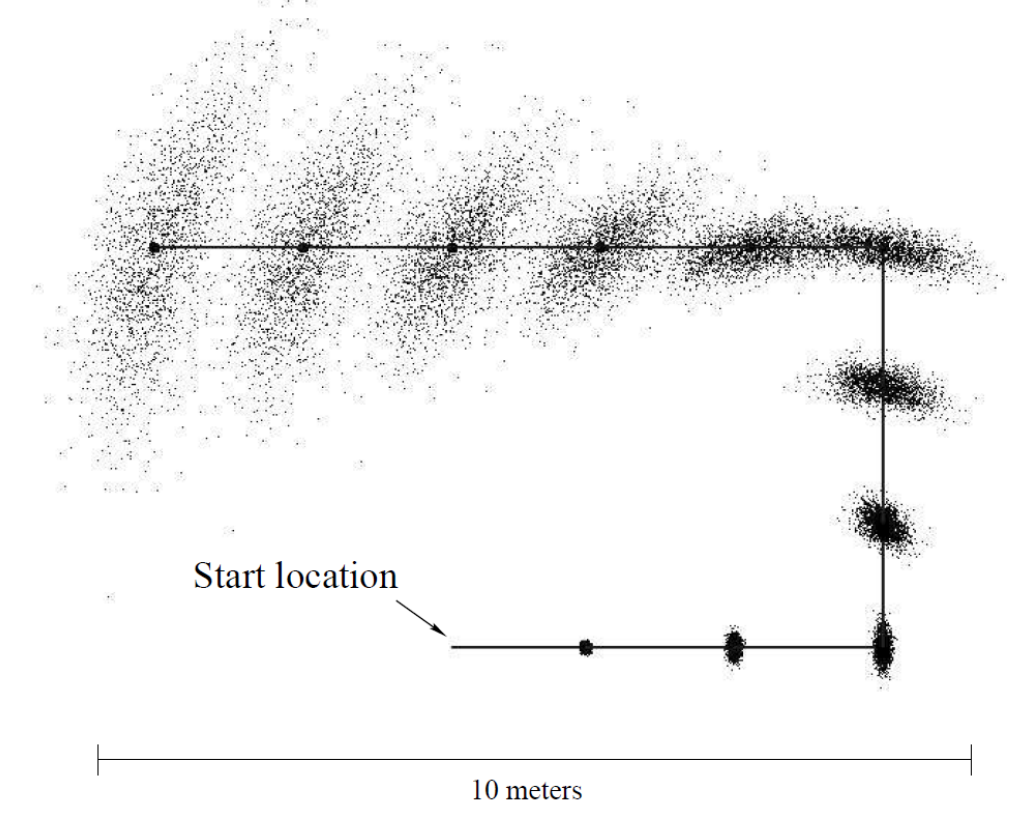
\includegraphics[width=0.4\textwidth]{images/unsure.png}
                    \caption{只用运动模型,误差不断累积}
                \end{figure}
\subsection{马尔可夫定位中的观测模型}
        \[
        p(\mathbf{x}_t \mid \mathbf{Z}^{t}, \mathbf{U}^{t-1}, \mathbf{m})
        = \eta \,\textcolor{red}{ p(\mathbf{z}_t \mid \mathbf{x}_t, \mathbf{m})}
        \int p(\mathbf{x}_t \mid \mathbf{x}_{t-1}, \mathbf{u}_{t-1}, \mathbf{m})
        \, p(\mathbf{x}_{t-1} \mid \mathbf{Z}^{t-1}, \mathbf{U}^{t-2}, \mathbf{m})
        \, d\mathbf{x}_{t-1}
        \]
        因为测量值=真实值+误差,我们希望同样利用误差分布进行建模。根据误差概率获得在$\mathbf{x}_t$观测到$\mathbf{z}_t$的可能性。由此来评估运动模型的$\mathbf{x}_t$是否准确。
    \begin{enumerate}
        \item \textbf{特征传感器模型和观测模型}
                    \begin{figure}[H]
                        \centering
                        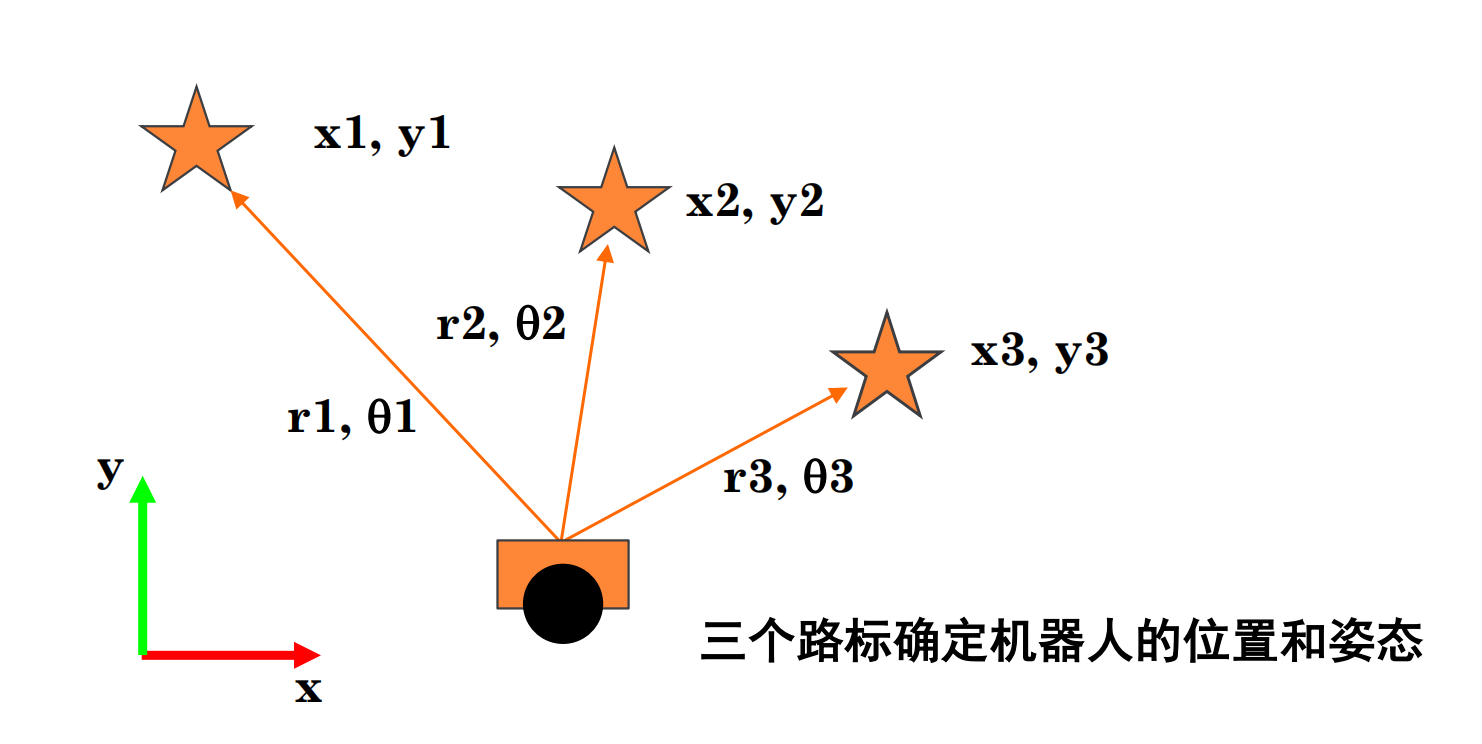
\includegraphics[width=0.6\textwidth]{images/3lubiao.png}
                        \caption{例如地图中存在三个物体,传感器对这三个物体分别观测其与机器人的距离$r$和夹角$\theta$,这两个变量相互独立且各自可建模为均值为0,标准差为$\sigma$的高斯分布}
                    \end{figure}
        
        \begin{enumerate}
            \item \textbf{定义}:
            \begin{itemize}
                \item 特征地图表示:$\mathbf{m}=\{\mathbf{m}_1,\mathbf{m}_2,\cdots,\mathbf{m}_N\}$\footnote{$\mathbf{m}_i$可以理解为每一个地图中的实际特征物体}, 在地图中的坐标为$\ (m_{ix},m_{iy})^{\mathsf T}$。
                \item $t$时刻的特征观测表示为:$\mathbf{z}_t=\{\,\mathbf{f}_t^{1},\mathbf{f}_t^{2},\ldots,\mathbf{f}_t^{K}\,\}$。
                \item $\mathbf{f}_t^{i}\triangleq\big(r_t^{i},\,\varphi_t^{i},\,s_t^{i}\big)^{\mathsf T}$
                \footnote{$\mathbf{f}_t^{i}$可以理解为机器人对每一个实际物体得到的测量特征}\\其中:
                \\$r_t^{i}$:特征与机器人之间的相对距离;
                \\$\varphi_t^{i}$:特征与机器人之间的相对角度;
                \\$s_t^{i}$:特征标识。
            \end{itemize}
        
            \item \textbf{观测独立}:假设每一个特征的观测条件独立,
            \[
                p(\mathbf{z}_t\mid \mathbf{x}_t,\mathbf{m})
                =p\!\big(\mathbf{f}_t^{1},\mathbf{f}_t^{2},\ldots,\mathbf{f}_t^{K}\mid \mathbf{x}_t,\mathbf{m}\big)
                =\prod_{k=1}^{K}p\!\big(\mathbf{f}_t^{k}\mid \mathbf{x}_t,\mathbf{m}\big).
            \]
        
            \item \textbf{特征的观测模型}\,$p(\mathbf{f}_t^{i}\mid \mathbf{x}_t,\mathbf{m})$:
            \begin{itemize}
                \item 假设$\mathbf{f}_t^{i}$对应的地图特征为$\mathbf{m}_j$,将地图特征$\mathbf{m}_j$转换到机器人坐标系下即为观测特征真值:
                \[
                \hat{\mathbf{f}}_t^{\,i}=
                \begin{pmatrix}
                    \sqrt{(m_{jx}-x)^2+(m_{jy}-y)^2}\\[2pt]
                    \operatorname{arctan2}(m_{jy}-y,\,m_{jx}-x)-\theta\\[2pt]
                    s_{j}
                \end{pmatrix},
                \qquad 
                \mathbf{x}_t=(x,\,y,\,\theta)^{\mathsf T}.
                \]
                \item 测量值$=$真实值$+$误差:$\mathbf{f}_t^{\,i}=\hat{\mathbf{f}}_t^{\,i}+\tilde{\boldsymbol\delta}_f$,且$\,\tilde{\delta}\sim\mathcal{N}(\delta;0,\sigma^{2})$\footnote{我们仍建模误差就是一个零均值、方差$\sigma^{2}$的高斯分布。};
                \item 根据观测误差模型,则
                \footnote{$\hat{\mathbf{f}}_t^{\,i}$是个常量,误差是个高斯分布的变量,两者加起来还是高斯分布}
                \[
                    p\!\big(\mathbf{f}_t^{i}\mid \mathbf{x}_t,\mathbf{m}\big)=\mathcal{N}\!\big(\mathbf{f}_t^{i};\,\hat{\mathbf{f}}_t^{\,i},\,\sigma_f^{2}\big).
                \]
            \end{itemize}
        \end{enumerate}
        
        \item \textbf{基于物理建模的激光束模型}

对于一次激光测量,可能遇到以下四种情况:
\begin{itemize}
    \item 正确测量(带有小测量噪声)
    \item 临时障碍\footnote{例如一个人走了过去}
    \item 未检测到物体
    \item 随机误差
\end{itemize}

那么我们可以将其观测模型拆解为以上四个部分:
\begin{flalign*}
& p\!\left(z_t^{k}\mid \mathbf{x}_t,\mathbf{m}\right)= &&
\end{flalign*}
$$
\alpha_{\mathrm{hit}}\,p_{\mathrm{hit}}\!\left(z_t^{k}\mid \mathbf{x}_t,\mathbf{m}\right)
+\alpha_{\mathrm{short}}\,p_{\mathrm{short}}\!\left(z_t^{k}\mid \mathbf{x}_t,\mathbf{m}\right)
+\alpha_{\mathrm{max}}\,p_{\mathrm{max}}\!\left(z_t^{k}\mid \mathbf{x}_t,\mathbf{m}\right)
+\alpha_{\mathrm{rand}}\,p_{\mathrm{rand}}\!\left(z_t^{k}\mid \mathbf{x}_t,\mathbf{m}\right),
$$
\vspace{1em}
其中,$\alpha_{\mathrm{hit}}+\alpha_{\mathrm{short}}+\alpha_{\mathrm{max}}+\alpha_{\mathrm{rand}}=1.$

\noindent 等价表达(对类别变量求和):
\[
p\!\left(z_t^{k}\mid \mathbf{x}_t,\mathbf{m}\right)
=\sum_{c} p\!\left(z_t^{k},c\mid \mathbf{x}_t,\mathbf{m}\right)
=\sum_{c} p\!\left(z_t^{k}\mid \mathbf{x}_t,\mathbf{m},c\right)p\!\left(c\mid \mathbf{x}_t,\mathbf{m}\right)
=\sum_{c} p\!\left(z_t^{k}\mid \mathbf{x}_t,\mathbf{m},\alpha\right)p(c),
\]
其中 $c\in\{\mathrm{hit},\mathrm{short},\mathrm{max},\mathrm{rand}\}$,且 $p(c)\in\{\alpha_{\mathrm{hit}},\alpha_{\mathrm{short}},\alpha_{\mathrm{max}},\alpha_{\mathrm{rand}}\}$。

具体而言,四部分模型可以分别进行建模:
\begin{enumerate}
    \item \textbf{带少量噪声的正确测量数据的概率模型}
    \begin{itemize}
        \item \textbf{建模思想}:可以被建模为真实距离的\textbf{高斯分布},其中真实距离可以通过\textbf{光线追踪算法}获得。
        \item \textbf{建模模型}:
        \[
        p_{\mathrm{hit}}\!\left(z_t^{k}\mid \mathbf{x}_t,\mathbf{m}\right)=
        \begin{cases}
            \eta\,\mathcal{N}\!\left(z_t^{k};\,z_{t}^{k*},\,\sigma_{\mathrm{hit}}^{2}\right), & 0\le z_t^{k}\le z_{\max},\\[2pt]
            0, & \text{otherwise},
        \end{cases}
        \qquad
        \]
        其中,
        \[\eta=\left(\displaystyle\int_{0}^{z_{\max}}\mathcal{N}\!\left(z;\,z_{t}^{k*},\,\sigma_{\mathrm{hit}}^{2}\right)\mathrm{d}z\right)^{-1}.
        \]
        用于归一化,确保概率积分后是1。\\
        此外:\\
        $z_{t}^{k*}$——通过光线追踪算法获得的真实距离;
        \\$z_{\max}$——最大测量距离。
        \begin{figure}[H]
            \centering
            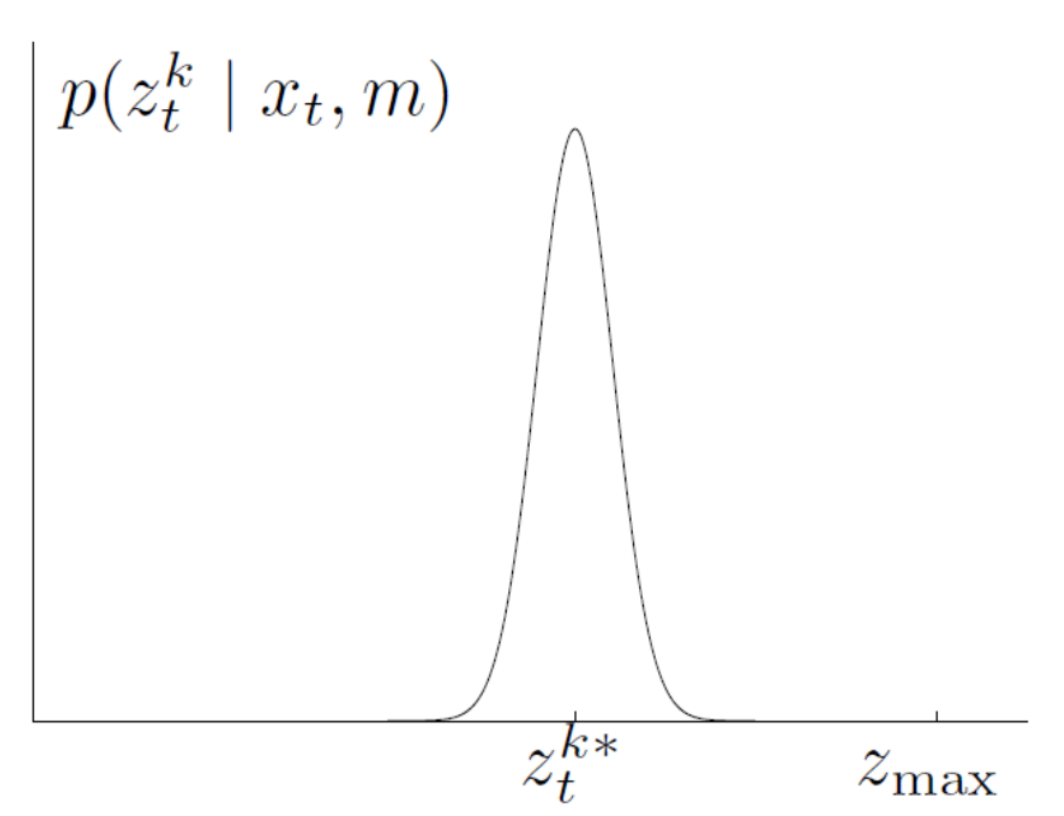
\includegraphics[width=0.35\linewidth]{images/guance1.png}
            \caption{带少量噪声的正确测量数据的概率模型(均值为真实距离的高斯分布)}
        \end{figure}
    \end{itemize}

    \item \textbf{临时障碍的测量数据的概率模型}
    \begin{itemize}
        \item \textbf{建模思想}:临时障碍往往导致测距仅得到非常短的数据,且随着距离的增大概率降低,因此可以建模为\textbf{截断的指数分布}。
        \item \textbf{建模模型}:
        \[
        p_{\mathrm{short}}\!\left(z_t^{k}\mid \mathbf{x}_t,\mathbf{m}\right)=
        \begin{cases}
            \eta\,\lambda_{\mathrm{short}}\,e^{-\lambda_{\mathrm{short}} z_t^{k}}, & 0\le z_t^{k}\le z_{t}^{k*},\\[2pt]
            0, & \text{otherwise},
        \end{cases}
        \qquad
        \]
        其中:
        \[
        \eta=\left(\displaystyle\int_{0}^{z_{t}^{k*}}\lambda_{\mathrm{short}} e^{-\lambda_{\mathrm{short}} z}\,\mathrm{d}z\right)^{-1}
        =(1-e^{-\lambda_{\mathrm{short}} z_{t}^{k*}})^{-1}.
        \]
        \begin{figure}[H]
            \centering
            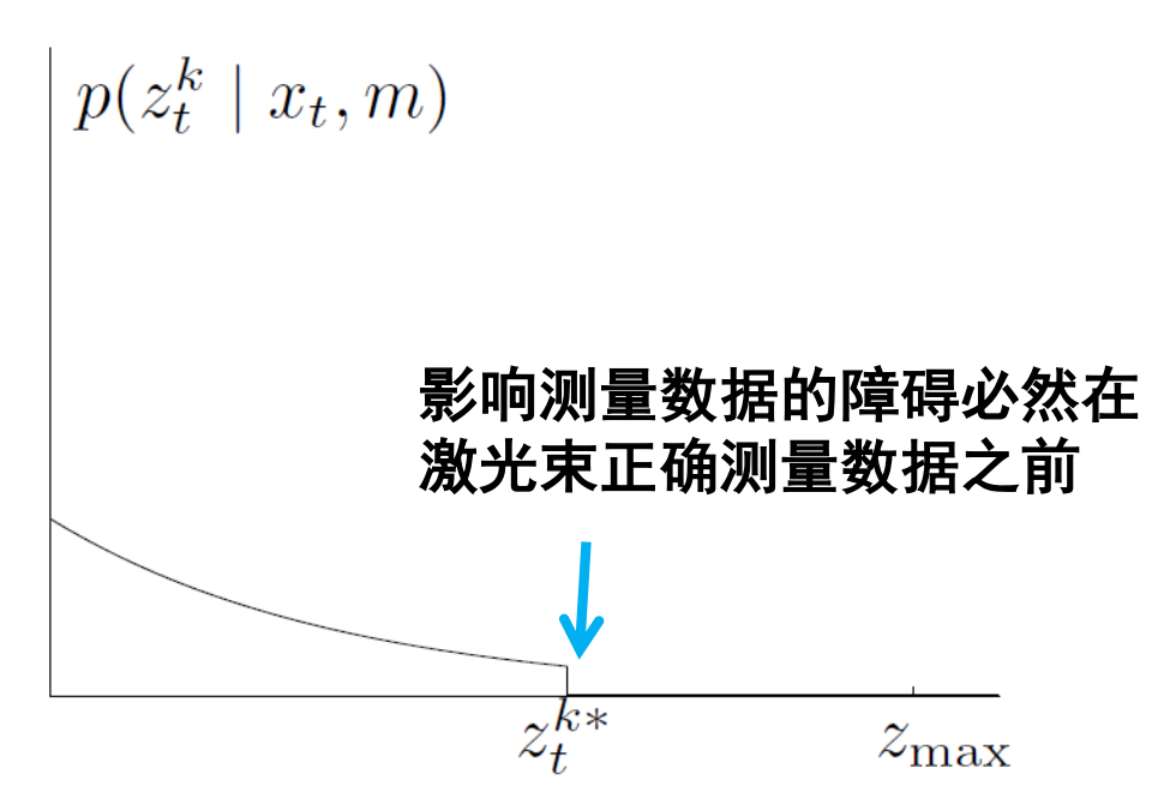
\includegraphics[width=0.35\linewidth]{images/guance2.png}
            \caption{临时障碍的测量数据的概率模型(截断的指数分布)}
        \end{figure}
    \end{itemize}

    \item \textbf{达到最大距离的测量数据的概率模型}
    \begin{itemize}
        \item \textbf{建模思想}:需要建模为一个伪概率分布,因为其数据只存在于一个值。
        \item \textbf{建模模型}:
        \[
        p_{\mathrm{max}}\!\left(z_t^{k}\mid \mathbf{x}_t,\mathbf{m}\right)=
        \begin{cases}
            1, & z_t^{k}=z_{\max},\\
            0, & \text{otherwise}.
        \end{cases}
        \]
        \begin{figure}[H]
            \centering
            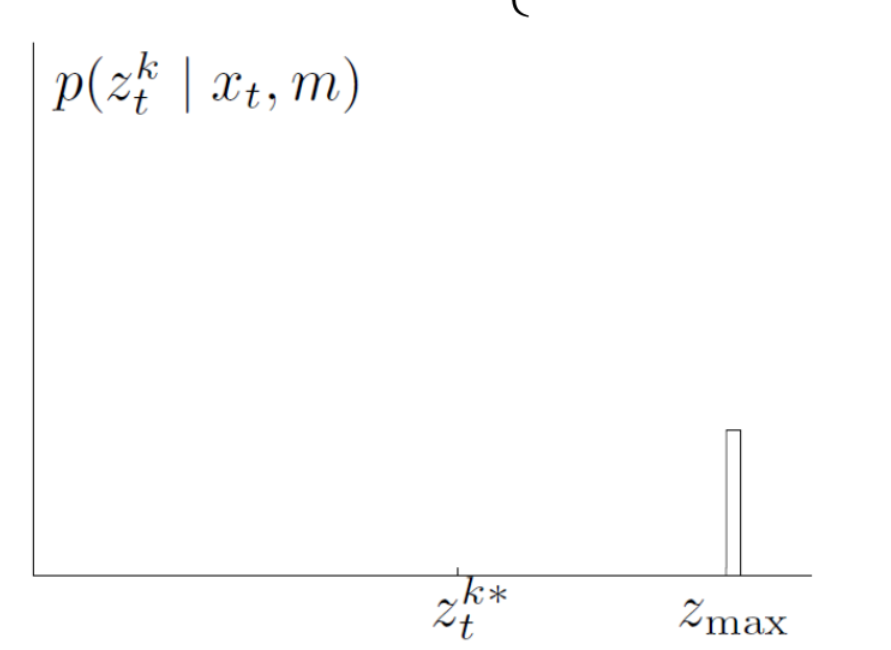
\includegraphics[width=0.35\linewidth]{images/guance3.png}
            \caption{达到最大距离的测量数据的概率模型(观测范围内恒为0)}
        \end{figure}
    \end{itemize}

    \item \textbf{随机错误测量数据的概率模型}
    \begin{itemize}
        \item \textbf{建模思想}:可以建模为\textbf{均匀分布},因为错误测量主要来自反射或串扰等传播问题,其机理建模较为复杂。
        \item \textbf{建模模型}:
        \[
        p_{\mathrm{rand}}\!\left(z_t^{k}\mid \mathbf{x}_t,\mathbf{m}\right)=
        \begin{cases}
            \dfrac{1}{z_{\max}}, & 0\le z_t^{k}<z_{\max},\\[6pt]
            0, & \text{otherwise}.
        \end{cases}
        \]
        \begin{figure}[H]
            \centering
            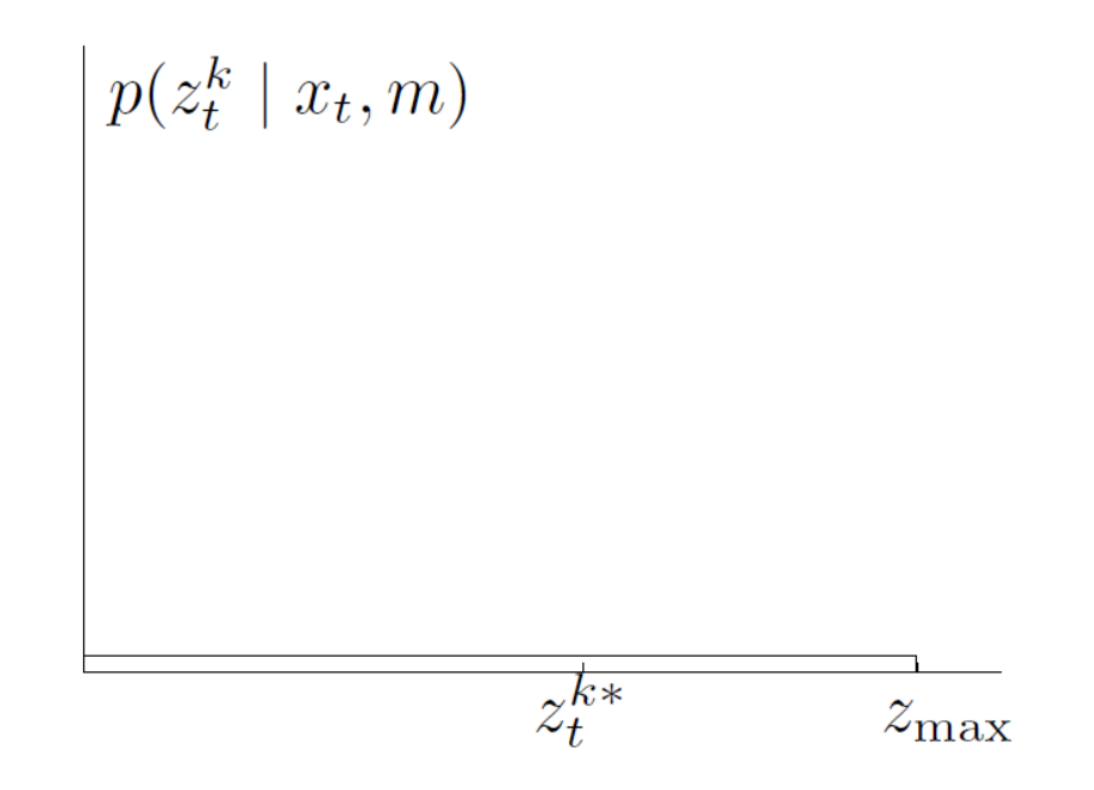
\includegraphics[width=0.35\linewidth]{images/guance4.png}
            \caption{随机错误测量数据的概率模型(均匀分布)}
        \end{figure}
    \end{itemize}
    合成以上四种模型,得到观测模型概率分布:
        \begin{figure}[H]
            \centering
            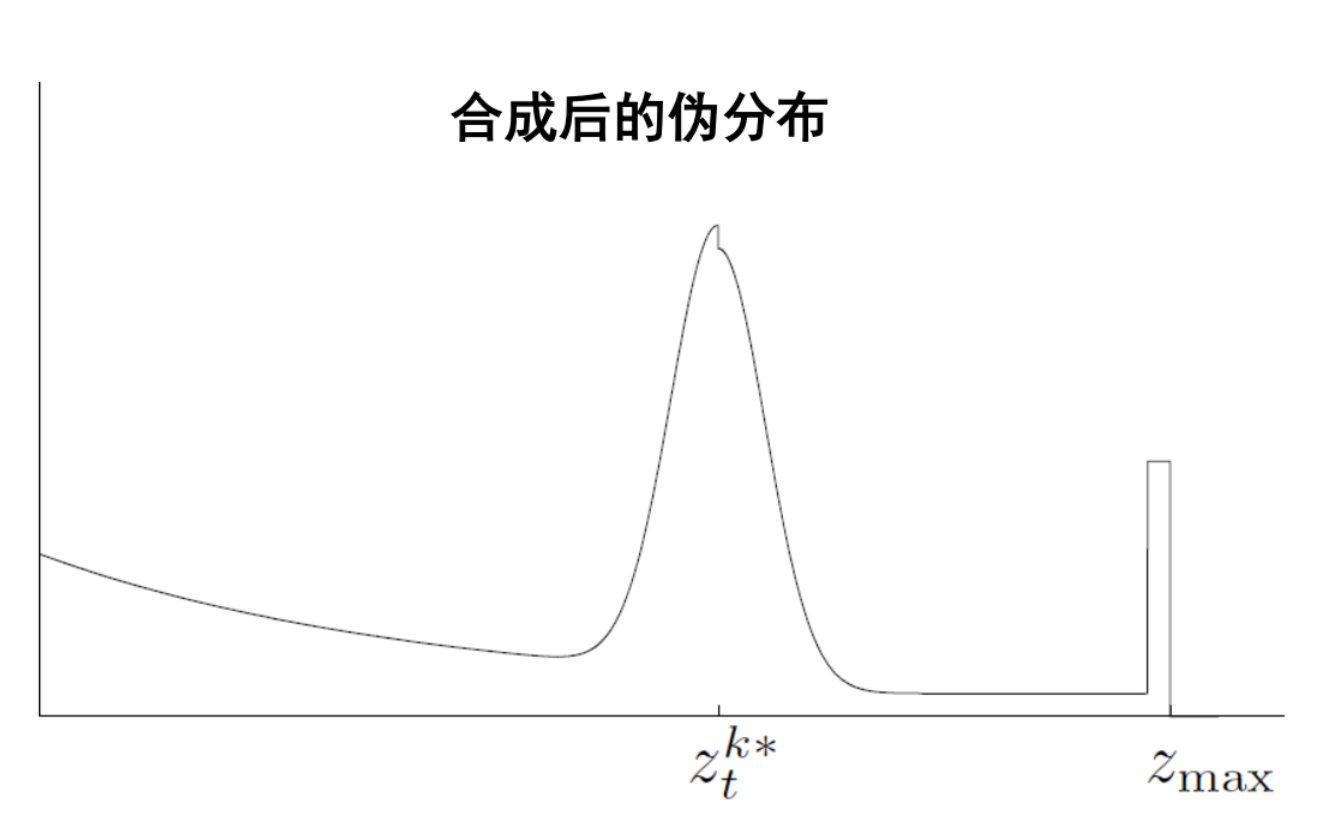
\includegraphics[width=0.35\linewidth]{images/guance5.png}
            \caption{基于物理建模的激光束模型四种模型合成后的伪分布}
        \end{figure}
\end{enumerate}
            \begin{itemize}
            \item \textbf{激光束模型参数确定}
            \begin{itemize}
                \item 模型中需要确定的参数
                \begin{itemize}
                    \item \textbf{概率分布本身的参数}
                    $\sigma_{\mathrm{hit}}^{2},\,\lambda_{\mathrm{short}}$
                    \item 四种数据模型混合的权值 $\alpha_{\mathrm{hit}},\,\alpha_{\mathrm{short}},\,\alpha_{\mathrm{max}},\,\alpha_{\mathrm{rand}}$
                \end{itemize}
                \item \textbf{参数确定方法}
                \begin{itemize}
                    \item 正常环境下,确定机器人的位置,给定一个与机器人距离已知的目标,然后利用激光测距仪测量目标,得到测量值,反复多次,得到大量数据样本
                    \item 根据样本,基于最大化样本集概率分布的思想,进行统计和学习
                \end{itemize}
                \item \textbf{数学描述}
                    \[
                    \max_{\Theta}\; p\!\left(\mathbf{Z}\mid \mathbf{X},\mathbf{m},\Theta\right),\qquad
                    \Theta=\left\{\sigma_{\mathrm{hit}}^{2},\,\lambda_{\mathrm{short}},\,\alpha_{\mathrm{hit}},\,\alpha_{\mathrm{short}},\,\alpha_{\mathrm{max}},\,\alpha_{\mathrm{rand}}\right\},
                    \]
                    
                    $\mathbf{Z}=\{z_i\}$ \text{为采集到的激光束样本集合}\\
                    $\mathbf{X}=\{\mathbf{x}_i\}$ \text{为对应的观测位姿集合}\\
                    $\mathbf{m}$ \text{为地图}.
                    
            \end{itemize}
                \item \textbf{优点}:
                \begin{itemize}
                    \item 物理意义非常明确
                    \item 对地图形式没有要求
                \end{itemize}
                \item \textbf{缺点}:
                \begin{itemize}
                    \item 计算:光线追踪算法耗时较大
                    \item 光滑性差:当地图中有很多小障碍物时,概率分布连续性很差,使得定位算法难以收敛
                \end{itemize}                
            \end{itemize}
 \item \textbf{基于LIKELIHOOD FIELD的激光束模型}
 \begin{itemize}
     \item \textbf{基本思想}:
     \begin{itemize}
         \item 把激光束末端投影于地图中
         \item 根据激光束末端投影与地图中最近物体之间距离建模
         \item 为减少在线计算量,根据地图离线构建Likelihood Field图
     \end{itemize}
        {\small\kaishu
        类似前面的运动模型的闭式求解与随机采样的正逆模型;\\
        \vspace{1em}
        光线追踪束模型:光线追踪给出应当的测距 $z_{t}^{k*}$,机器人获得观测 $z_t^k$,用$\alpha_{\mathrm{hit}},\alpha_{\mathrm{short}},\alpha_{\mathrm{max}},\alpha_{\mathrm{rand}}$
        的混合分布为不同观测值赋予概率,从而评估“观测成这样有多合理”;\\
        \vspace{1em}
        Likelihood Field:直接把观测 $z_t^k$ 沿该束方向在位姿 $\mathbf{x}_t$ 下投影到地图端点
        $\mathbf{p}_{t}^{k}$,查询预先计算好的距离场 $D(\cdot)$ 得到
        $d=D(\mathbf{p}_{t}^{k})$,并用
        $p(z_t^k\mid\mathbf{x}_t,\mathbf{m})\propto\exp(-d^{2}/2\sigma^{2})$
        评估“观测成这样有多合理”(各束条件独立时取乘积)。}
    \begin{figure}[H]
        \centering
        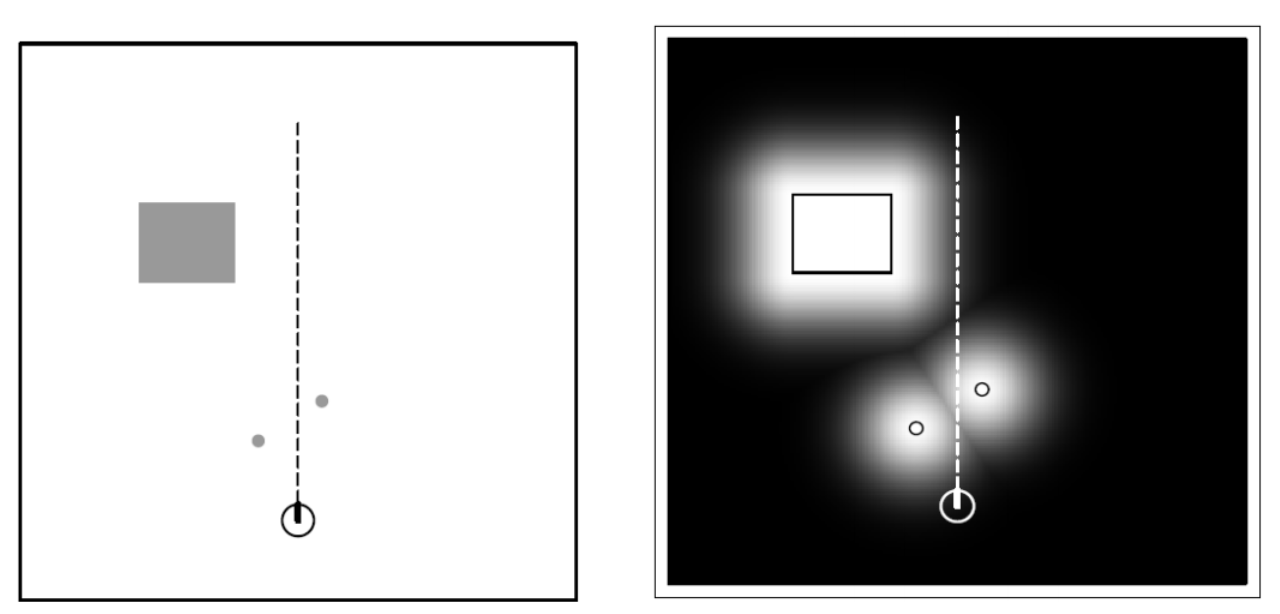
\includegraphics[width=0.5\linewidth]{images/Likelyhood.png}
        \caption{likelihood field图(右),白色表示概率高}
    \end{figure}
    \begin{enumerate}
      \item \textbf{概率描述}:
      \[
      p\!\left(z_t^{k}\mid \mathbf{x}_t,\mathbf{m}\right)
      =\alpha_{\mathrm{hit}}\,p_{\mathrm{hit}}\!\left(z_t^{k}\mid \mathbf{x}_t,\mathbf{m}\right)
      +\alpha_{\mathrm{max}}\,p_{\mathrm{max}}\!\left(z_t^{k}\mid \mathbf{x}_t,\mathbf{m}\right)
      +\alpha_{\mathrm{rand}}\,p_{\mathrm{rand}}\!\left(z_t^{k}\mid \mathbf{x}_t,\mathbf{m}\right),
      \]
      其中:\\
      $\alpha_{\mathrm{hit}}+\alpha_{\mathrm{max}}+\alpha_{\mathrm{rand}}=1$\\
      $z_t^{k}$——一次激光测量的数据;\\
      因无法考虑临时障碍物(预先建图),所以取消
      $p_{\mathrm{short}}\!\left(z_t^{k}\mid \mathbf{x}_t,\mathbf{m}\right)$。
    
      \item \textbf{末端投影距离建模}\\
      \,$p_{\mathrm{hit}}\!\left(z_t^{k}\mid \mathbf{x}_t,\mathbf{m}\right)$:
      记 $z_t^{k}$ 末端在地图中的坐标为 $\bigl(x_{z_t^{k}},y_{z_t^{k}}\bigr)^{\mathsf T}$,
      寻找地图中与该坐标最近的物体,计算两者间距
      \[
      \mathrm{dist}=\arg\min_{\ (m_x,m_y)\ \text{is occupied in map}}
      \sqrt{(m_x-x_{z_t^{k}})^{2}+(m_y-y_{z_t^{k}})^{2}},
      \]
      \[
      p_{\mathrm{hit}}\!\left(z_t^{k}\mid \mathbf{x}_t,\mathbf{m}\right)=\mathcal{N}\!\left(\mathrm{dist};\,0,\,\sigma^{2}\right).
      \]
    
    
      \item \textbf{基于栅格地图的\;LIKELIHOOD FIELD\;建立}:
      预先建立。对于栅格地图中的每一个未占用栅格,搜索距离最近的占用栅格,计算高斯分布下的概率赋给该未占用栅格\footnote{%
\textbf{距离场(offline)}\;先对占据栅格地图做欧氏距离变换(EDT),得每个栅格到最近障碍物的距离
\[
d(\mathbf{c})=\min_{\mathbf{o}\in\mathcal{O}}\;\lVert \mathbf{c}-\mathbf{o}\rVert_2 .
\]
\textbf{似然场(由距离场映射)}\;用零均值高斯核把“越靠近障碍物越合理”转为命中似然
\[
p_{\mathrm{hit}}(\mathbf{c})=\eta\,\exp\!\Big(-\tfrac{d(\mathbf{c})^2}{2\sigma^2}\Big),
\quad
\eta^{-1}=\!\!\sum_{\mathbf{c}}\exp\!\Big(-\tfrac{d(\mathbf{c})^2}{2\sigma^2}\Big).
\]
\textbf{在线评估}\;把激光端点投到地图坐标 $\mathbf{p}$,查表 $p_{\mathrm{hit}}(\mathbf{p})$,再与
\[
p_{\mathrm{max}}(z)=\mathbb{I}[z=z_{\max}],\qquad
p_{\mathrm{rand}}(z)=\begin{cases}1/z_{\max},&0\le z<z_{\max},\\[2pt]0,&\text{otherwise}\end{cases}
\]
按权重混合即可:
\[
p\!\left(z_t^{k}\mid \mathbf{x}_t,\mathbf{m}\right)=
\alpha_{\mathrm{hit}}\,p_{\mathrm{hit}}(\mathbf{p})
+\alpha_{\mathrm{max}}\,p_{\mathrm{max}}(z_t^{k})
+\alpha_{\mathrm{rand}}\,p_{\mathrm{rand}}(z_t^{k}),
\quad \alpha_{\mathrm{hit}}+\alpha_{\mathrm{max}}+\alpha_{\mathrm{rand}}=1.
\]
}%
,最后给未知栅格赋值 $1/z_{\max}$。
    
      \item \textbf{基于\;LIKELIHOOD FIELD\;的激光束模型}:
      图中激光束的正确测量传感器概率分布 $p_{\mathrm{hit}}\!\left(z_t^{k}\mid \mathbf{x}_t,\mathbf{m}\right)$;
      结合最大测量和随机误差模型后的概率分布
      $p\!\left(z_t^{k}\mid \mathbf{x}_t,\mathbf{m}\right)$。

    \end{enumerate}
\end{itemize}
    \begin{itemize}
        \item \textbf{优点}:
        \begin{itemize}
            \item 在线计算量小;
            \item 平滑性好\footnote{基于物理建模的激光束模型的高斯分布是在\textbf{激光束方向}上,隐含的假设是物体的不确定性只存在于激光束方向上,满足激光束测量的物理意义,但造成平滑性非常差;基于\emph{Likelihood Field} 的激光束模型的高斯分布是在\textbf{障碍物周围},即假设障碍物的不确定性遍布它的四周,更符合实际情况。},可确保算法收敛\footnote{物理束模型沿射线与栅格/遮挡相交会产生大量不连续跳变,目标面粗糙、梯度差,优化/滤波更易发散或不收敛。}
        \end{itemize}
        \item \textbf{缺点}:
        \begin{itemize}
            \item 没有明确的物理意义;
            \item 无法建模人等临时动态障碍造成的错误测量,适用于人流较少时的实际应用。
        \end{itemize}
          
      
    
     
    



 \end{itemize}




            
\end{enumerate}
\end{document}